
\chapter{Experimental results}

\section{Proof-of-concept design}

\subsection{Geometry and parameters}

The first sample that was measured was created from a proof-of-concept design, which was aimed at testing general properties of the simplest Xmon-based cQED systems. The easiest way to gain insight about the structure of the sample is to look at \autoref{fig:first_chip_design_full} where some of the main parts of its design are shown. The chip is 8 mm long and 4 mm wide and consists basically of six isolated qubit-resonator systems. 

All of the resonators were $\lambda/4$ with frequencies designed to be $6, 6.5, 6.9,7,7.1,8$ GHz for devices I-VI, respectively. Their coplanar parameters are $7\,\mu$m for the central wire width and $4\,\mu$m for the gaps.

The qubits were designed to be identical, with $C_\Sigma \approx 80$ fF and $I_{C, \Sigma} = 60$ nA, giving the $\omega_{01}/2\pi \approx 7$ GHz at their flux sweet-spot ($\Phi_{ext}=0$) and anharmonicity of approximately $-230$ MHz.

Two test structures at the sides of the chip were also included to allow direct DC measurement of the SQUIDs created during the shadow evaporation.

\subsection{Purposes and implementation}

The main targets for the chip were:
\begin{enumerate}[label=(\alph*), leftmargin=1.5cm]
\itemsep0pt
 \item to check the measurement setup
 \item to check the calculations for the frequencies and the coupling strengths
 \item to roughly check the coherence of Xmons
 \item to estimate the reproducibility of the junctions 
 \item to observe the AC-Stark shift 
 \item to observe high-power multiphoton transitions and sidebands
 \item to check for the interesting effects caused by different resonator detunings at sweet-spot  
\end{enumerate}

\begin{figure}[h!]
\centering
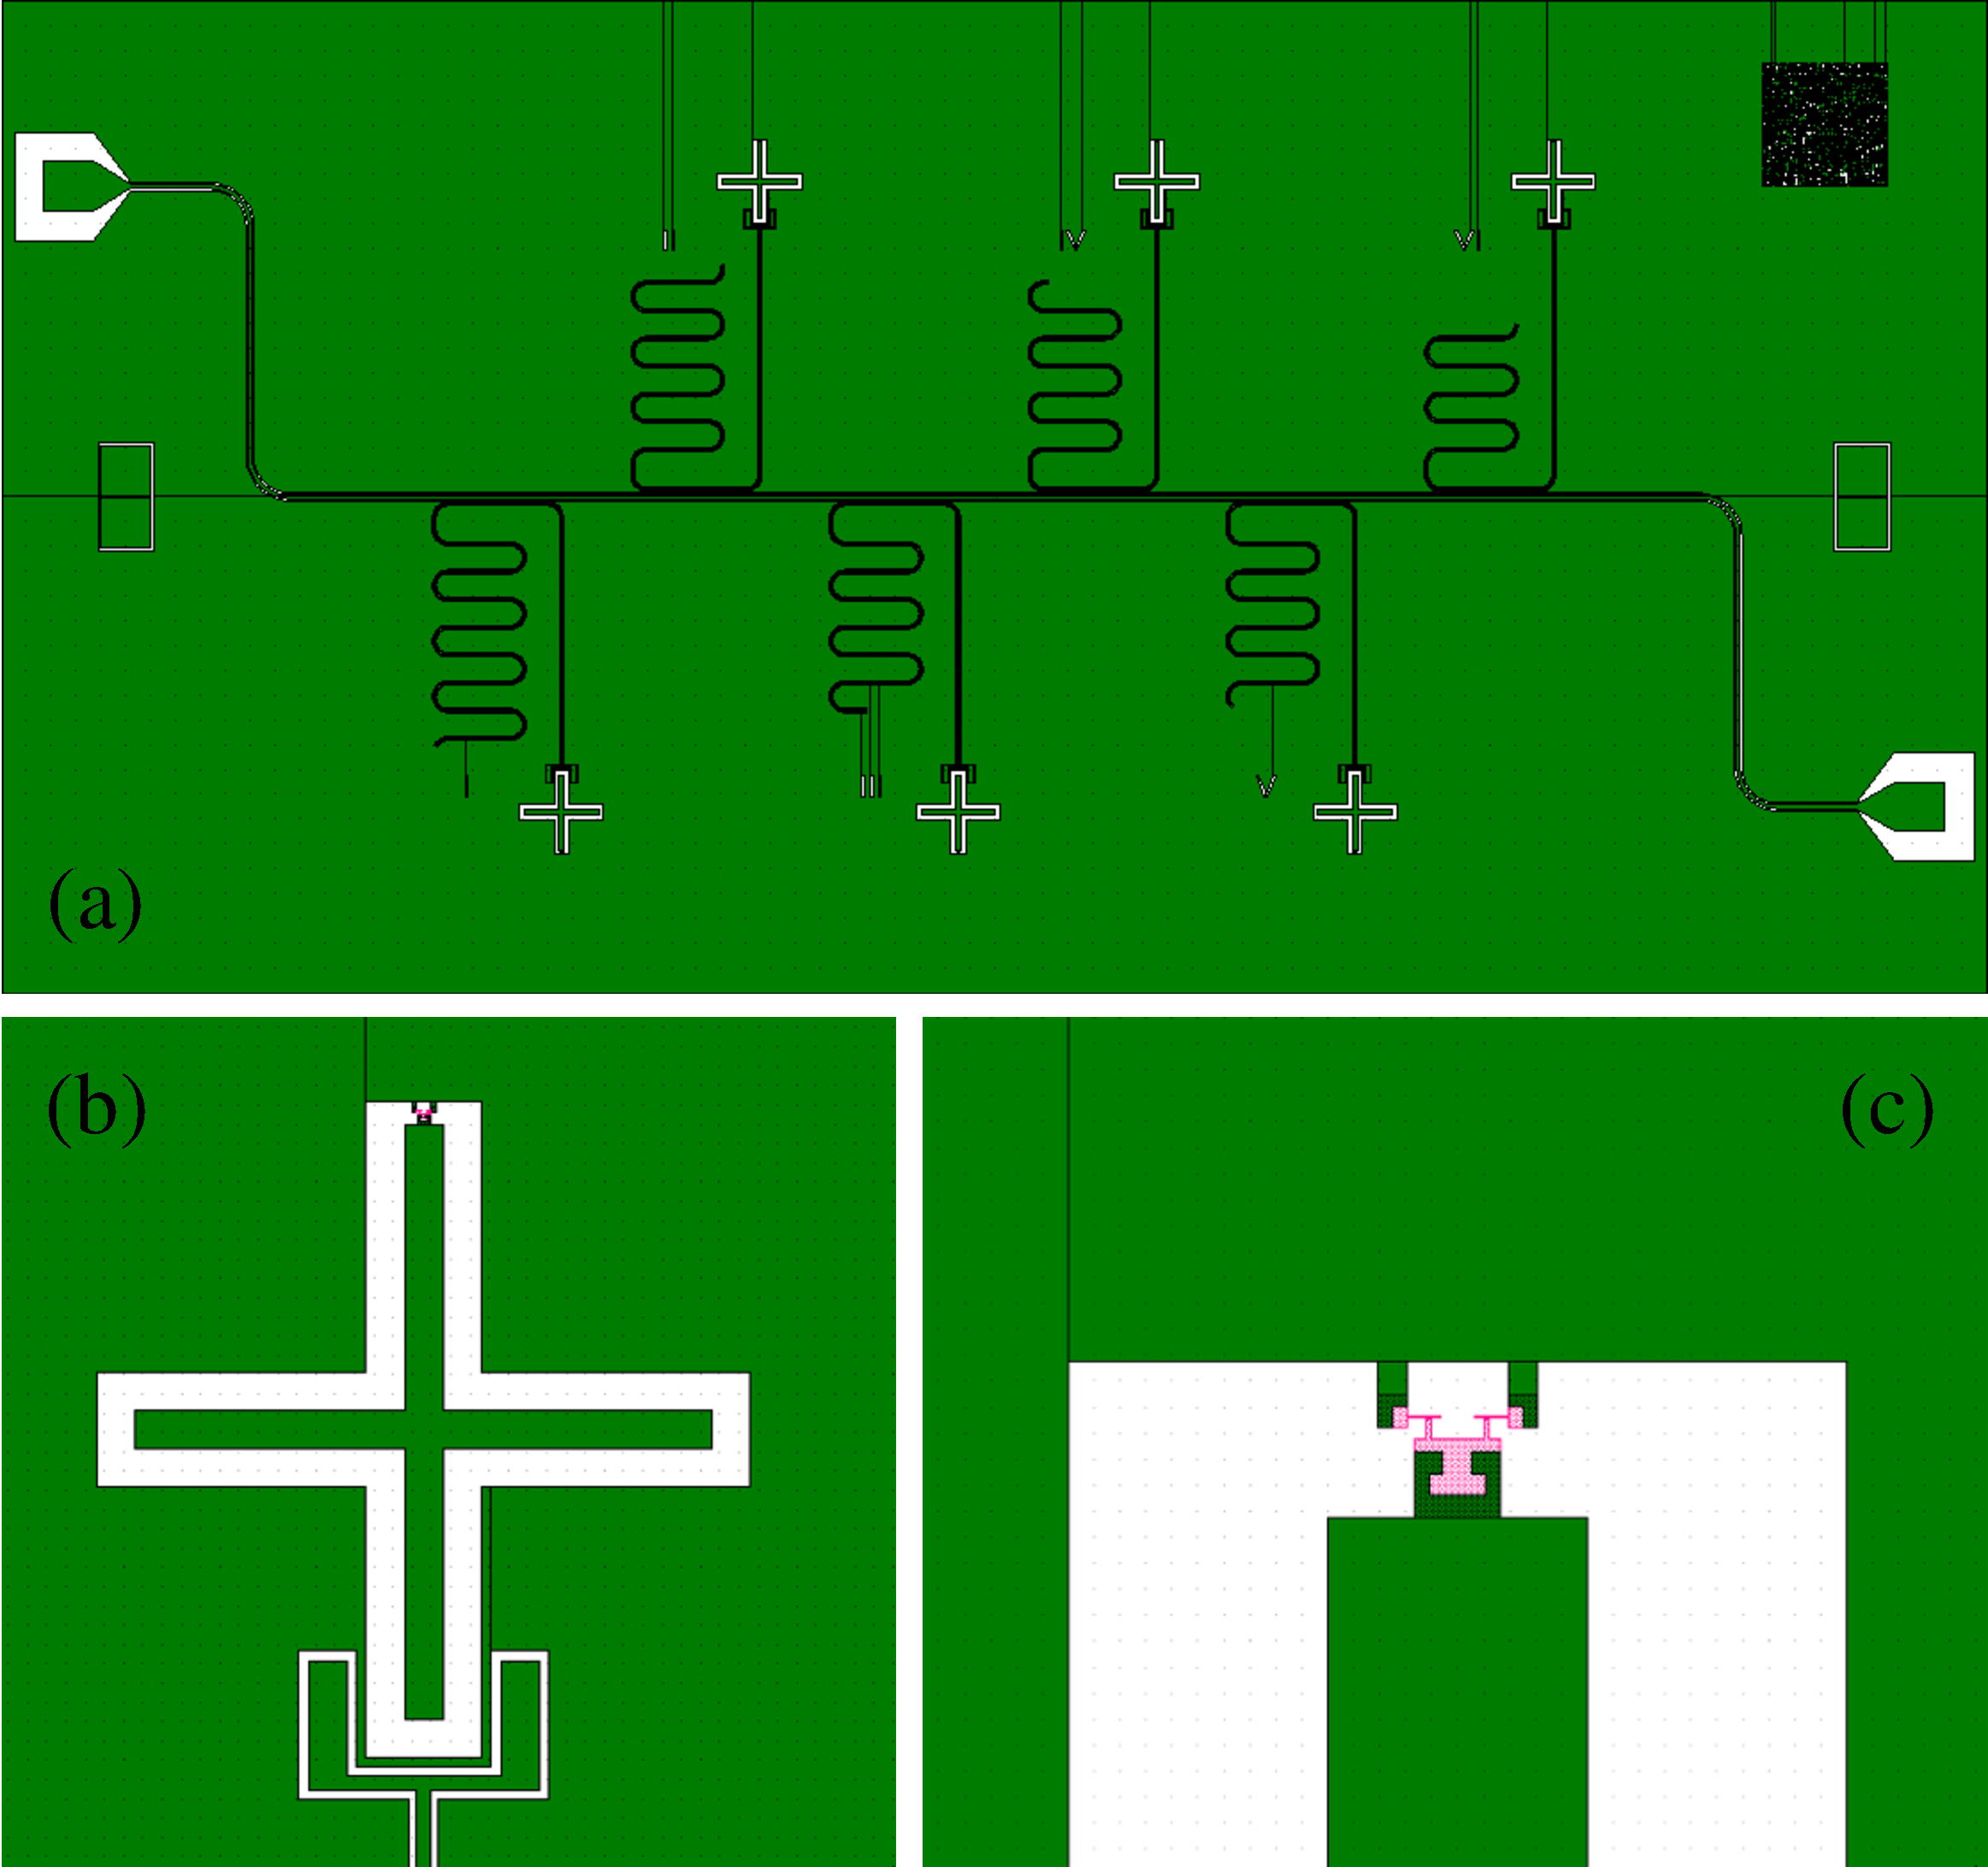
\includegraphics[width=0.9\textwidth]{chip_design_full}
\caption{\textbf{(a)} Large-scale image of the design used for the proof-of-concept sample. The chip (8x4 mm) consists of six $\lambda/4$ CPW resonators coupled capacitively to the feedline each with an Xmon qubit at the open end. \textbf{(b)} Zoomed area around one of the qubits, showing its cross-shaped capacitor and the ``claw'' coupler of its resonator. \textbf{(c)} Zoom around one of the qubits' SQUIDs. Pink areas denote the e-beam mask that was used for shadow evaporation.}
\label{fig:first_chip_design_full}
\end{figure}

The sample was fabricated in the cleanroom facility at MIPT, in a two-step process. Firstly, electron beam lithography was used to form the shadow evaporation mask for the pads with junctions and Al was shadow evaporated on the Plassys unit ($\pm 7^\circ$). Secondly, the photolithograpy was used to pattern larger structures like the feedline, resonators and Xmons' capacitors aligned with e-beam lithography and finally another layer of Al was deposited.	

\begin{figure}
\centering
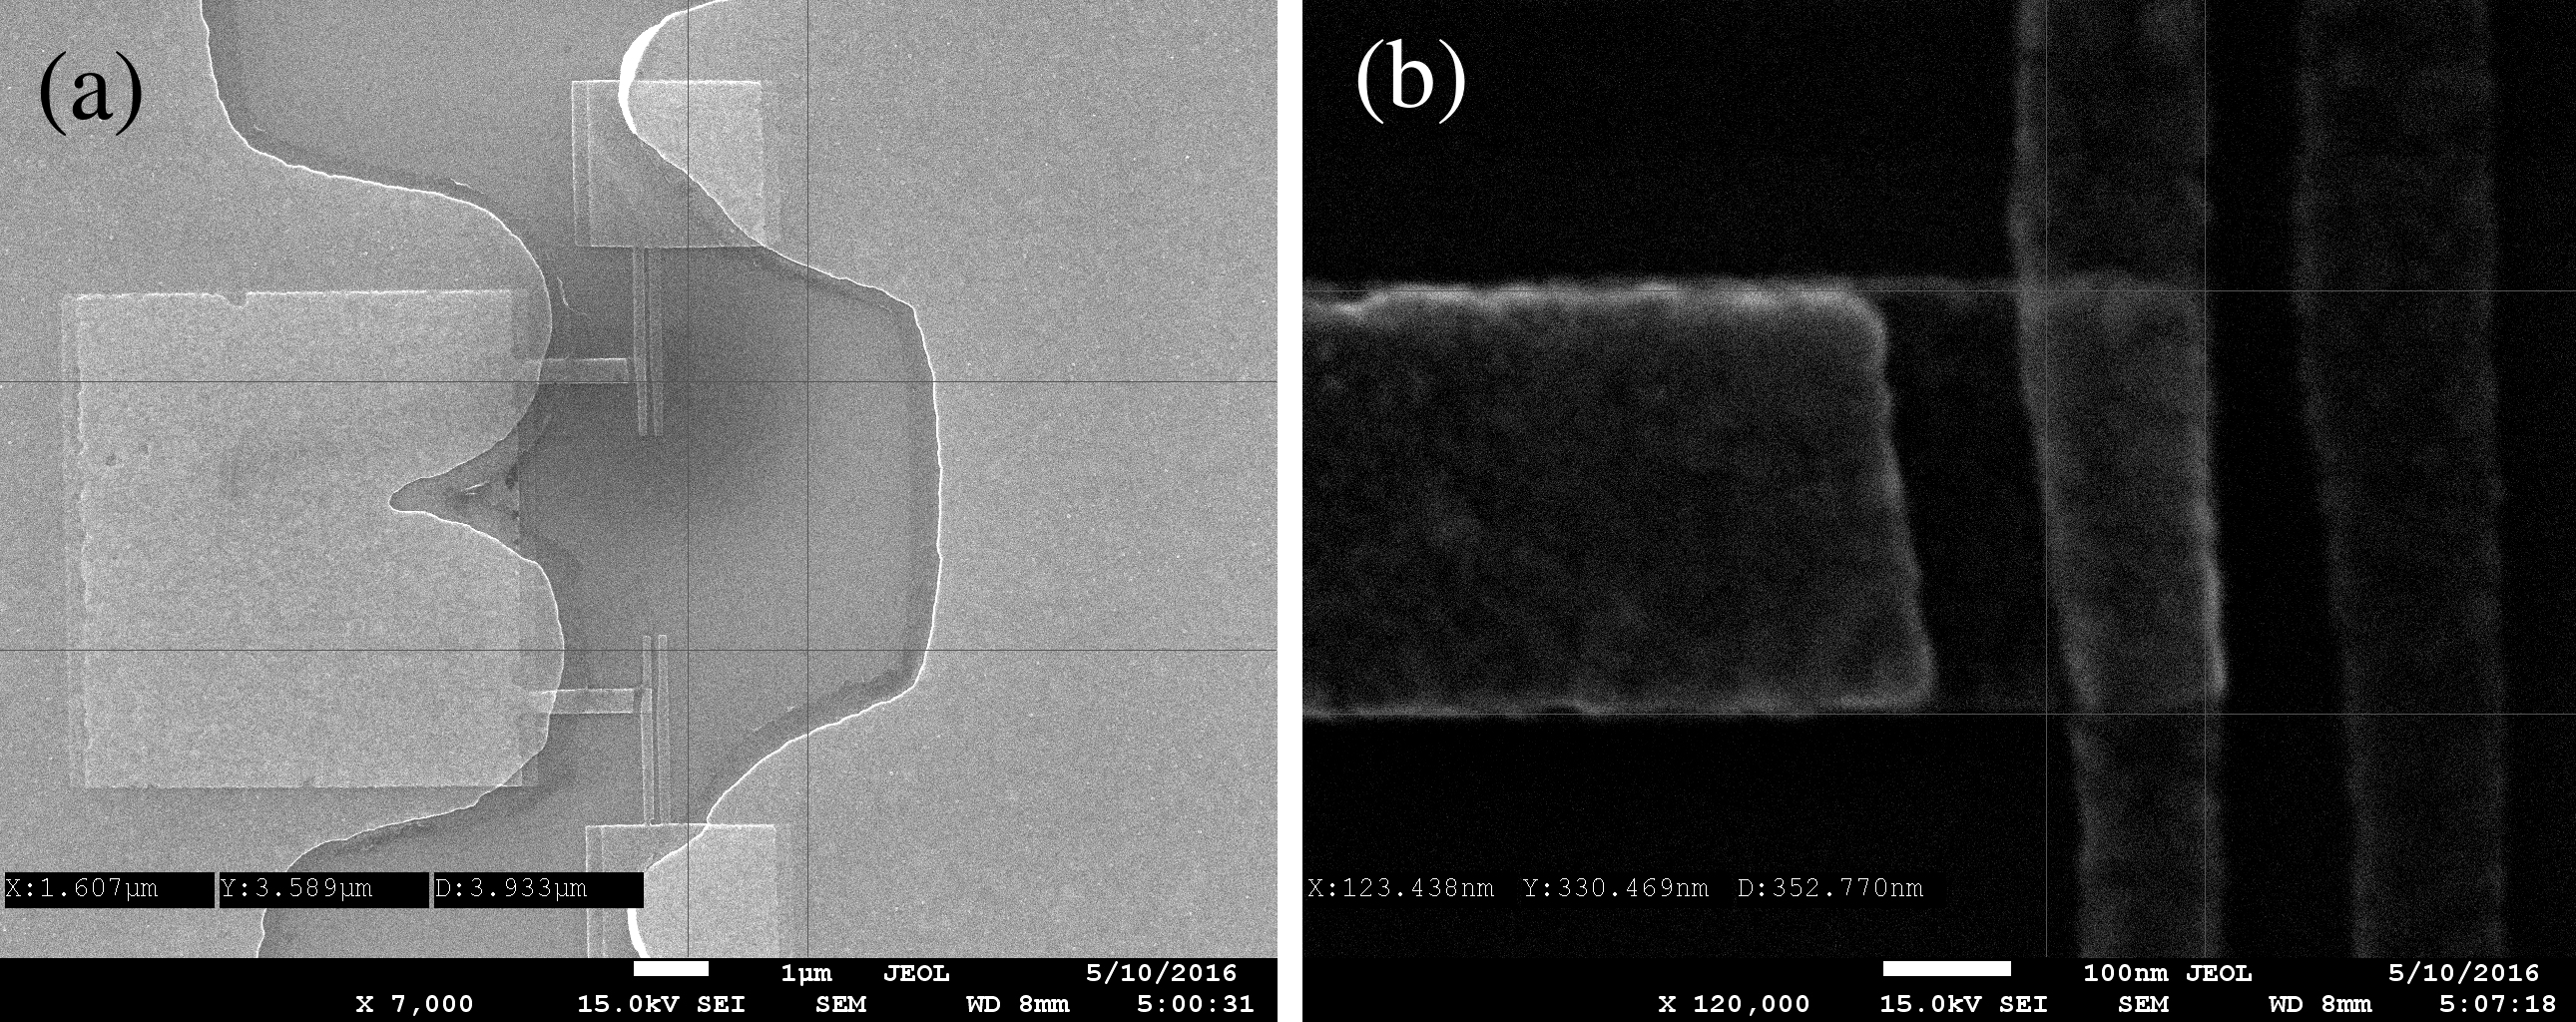
\includegraphics[width=0.9\textwidth]{X_mon_JJ_SQUID}
\caption{\textbf{(a)} SEM micrograph of the SQUID of one of the test structures on the chip. One can see that photo- and electron lithography are aligned, however fine structures \autoref{fig:first_chip_design_full}~(c) were not resolved during the second step. \textbf{(b)} Enlarged view on one of the junctions (upper). Its area is approximately $120\times 330\approx 0.4\, \mu m^2$, in the design it's $0.3\,\mu m^2$.} 
\end{figure}

\subsection{Measurement setup}

The sample was measured at ISSP in laboratory of RQC. Cryogenic equipment was represented by BlueFors LD250 dilution refrigerator, with base temperature of 16 mK. The microwave equipment included R\&S ZNB 10 kHz-20 GHz vector network analyser,  Agilent E8257D 100 kHz - 40 GHz analog signal generator. The sample was flux biased using Keithley 6221 current source.

Microwave line was thermalized with 60 dB of attenuation, additional 20 dB of attenuation were introduced on a directional coupler which added the second tone from the $\mu$-wave source. After leaving the sample the signal passed through two isolators and a hybrid coupler, which was used before to measure two samples during single cooldown. Finally, the signal was amplified with 4-8 GHz LNF amplifier at 4 K and a with a room-temperature amplifier.

The sample holder that was used was designed for 10x10 mm chips, so the bondwires had a relatively large length of 1 mm which of course deteriorated the overall transmission. Chip lay directly on the copper disk of the bottom part of the sample holder with no hole carved under it. Around the sample holder a superconducting coil was wound which has been supplied using the current source mentioned above.

The magnetic shielding of the sample holder was achieved via a cryoperm shield. A superconducting shield was not installed in this run due to the lack of space inside the magnetic shield, which may have influenced the noise background.


\subsection{Characterization of the resonators}

As a first step of characterizing the sample a study of the resonances was performed. In \autoref{fig:first_resonators_general} the power transmission through the cryostat is shown. In can be seen that in overall the transmission level is at approximately $-35$ dB. As long as the amplifiers add 60 dB the directional coupler and the hybrid coupler subtract 23 dB, it can be inferred that the sample in the sampleholder itself has approximately -10 dB transmission. This should be improved with better impedance matching to reduce noise. Secondly, there is a clear 300 MHz-wide dip in the transmission around 6.2 GHz, which should also be eliminated.

\begin{figure}[h]
\centering
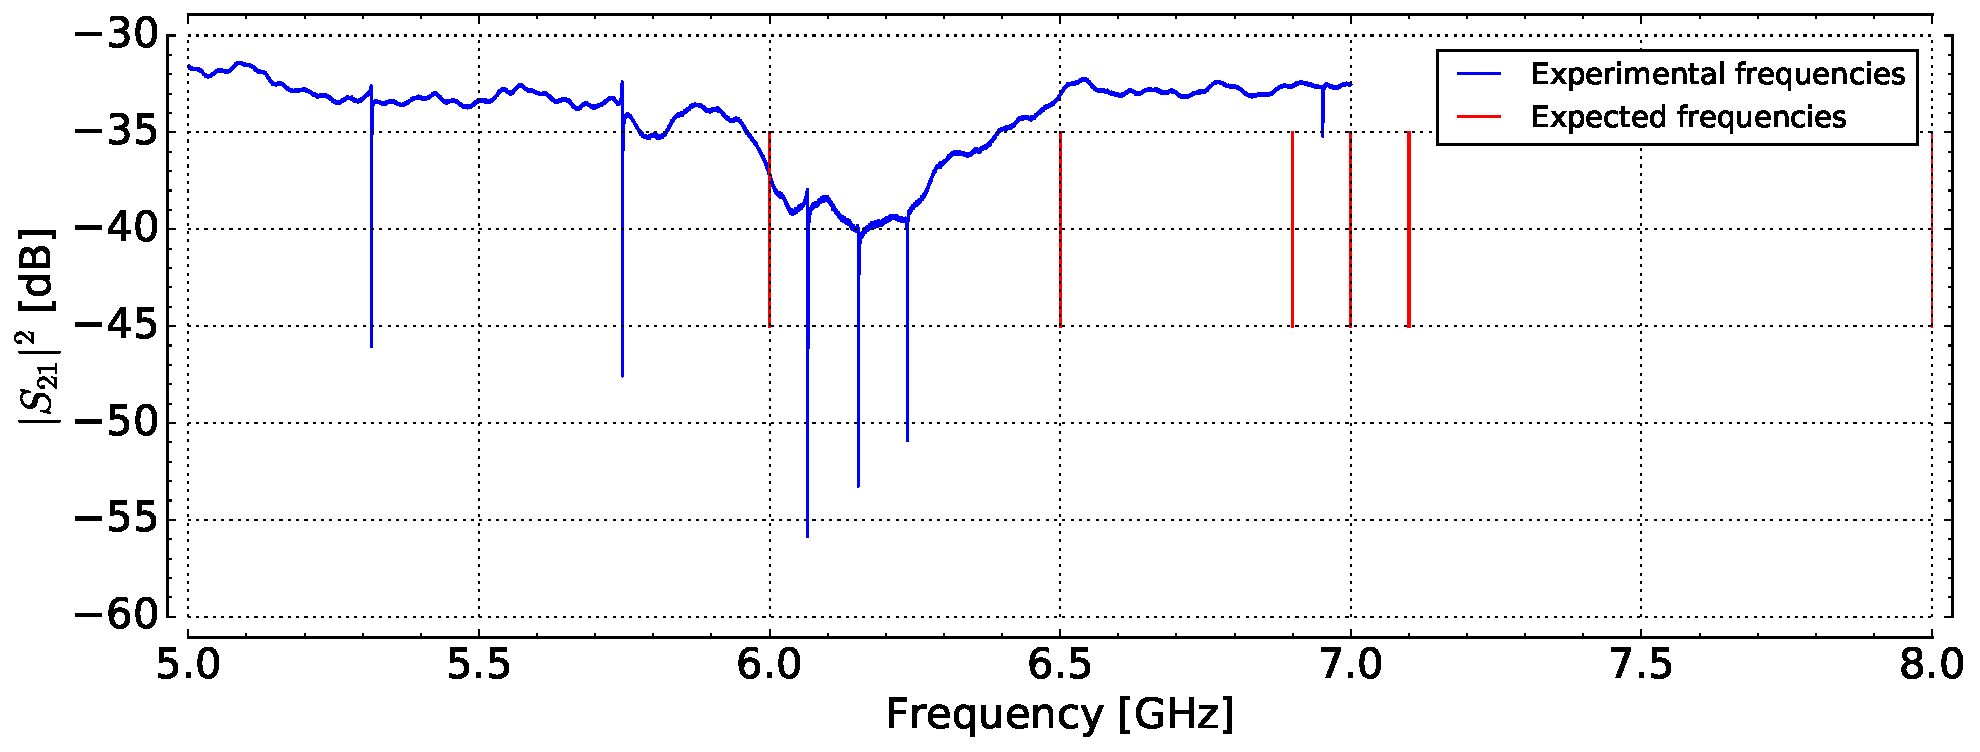
\includegraphics[width=\textwidth]{xmon-first-try_general15x5}
\caption{General view of the resonances. All six resonances are visible, however shifted far down in frequency. This shift is due to a mistake in the design which didn't compensate for the ``claw'' couplers at the resonator ends.}
\label{fig:first_resonators_general}
\end{figure}

All resonators are functional which can be seen from the presence of six sharp dips in transmission. The frequencies at which the dips occur are significantly lower than expected because there was a flaw in the macro code which draws the design. The frequency compensation routine made specifically to calculate the frequency shift\cite{Sank2014} caused by the ``claw'' coupler at the end of the resonator was not executed, so the length of the resonators became larger than it should have been. At higher frequencies the phase shift of the ``claw'' is larger so the frequency discord is larger there.

Below the results obtained using the \textit{circlefit}\cite{probst2015} fitting method are presented. Each peak from \autoref{fig:first_resonators_general} was enlarged and scanned with a fine resolution and averaged to reduce noise (more averages on low and less on high powers). Then for each power complex $S_{21}$ data for each scan area around a resonance was recorded.

After all of the data had been obtained, the fitting procedure has been applied for every scan at each power. The full fitting process is described in depth in the original publication\cite{probst2015}. In practice the whole algorithm is encapsulated in several function calls of the library called \textit{resonator tools} that the authors have kindly provided via \href{https://github.com/sebastianprobst/resonatortools}{GitHub}. Fitting results are summarized in \autoref{fig:first_q_factors}.

\begin{figure}[t]
\centering
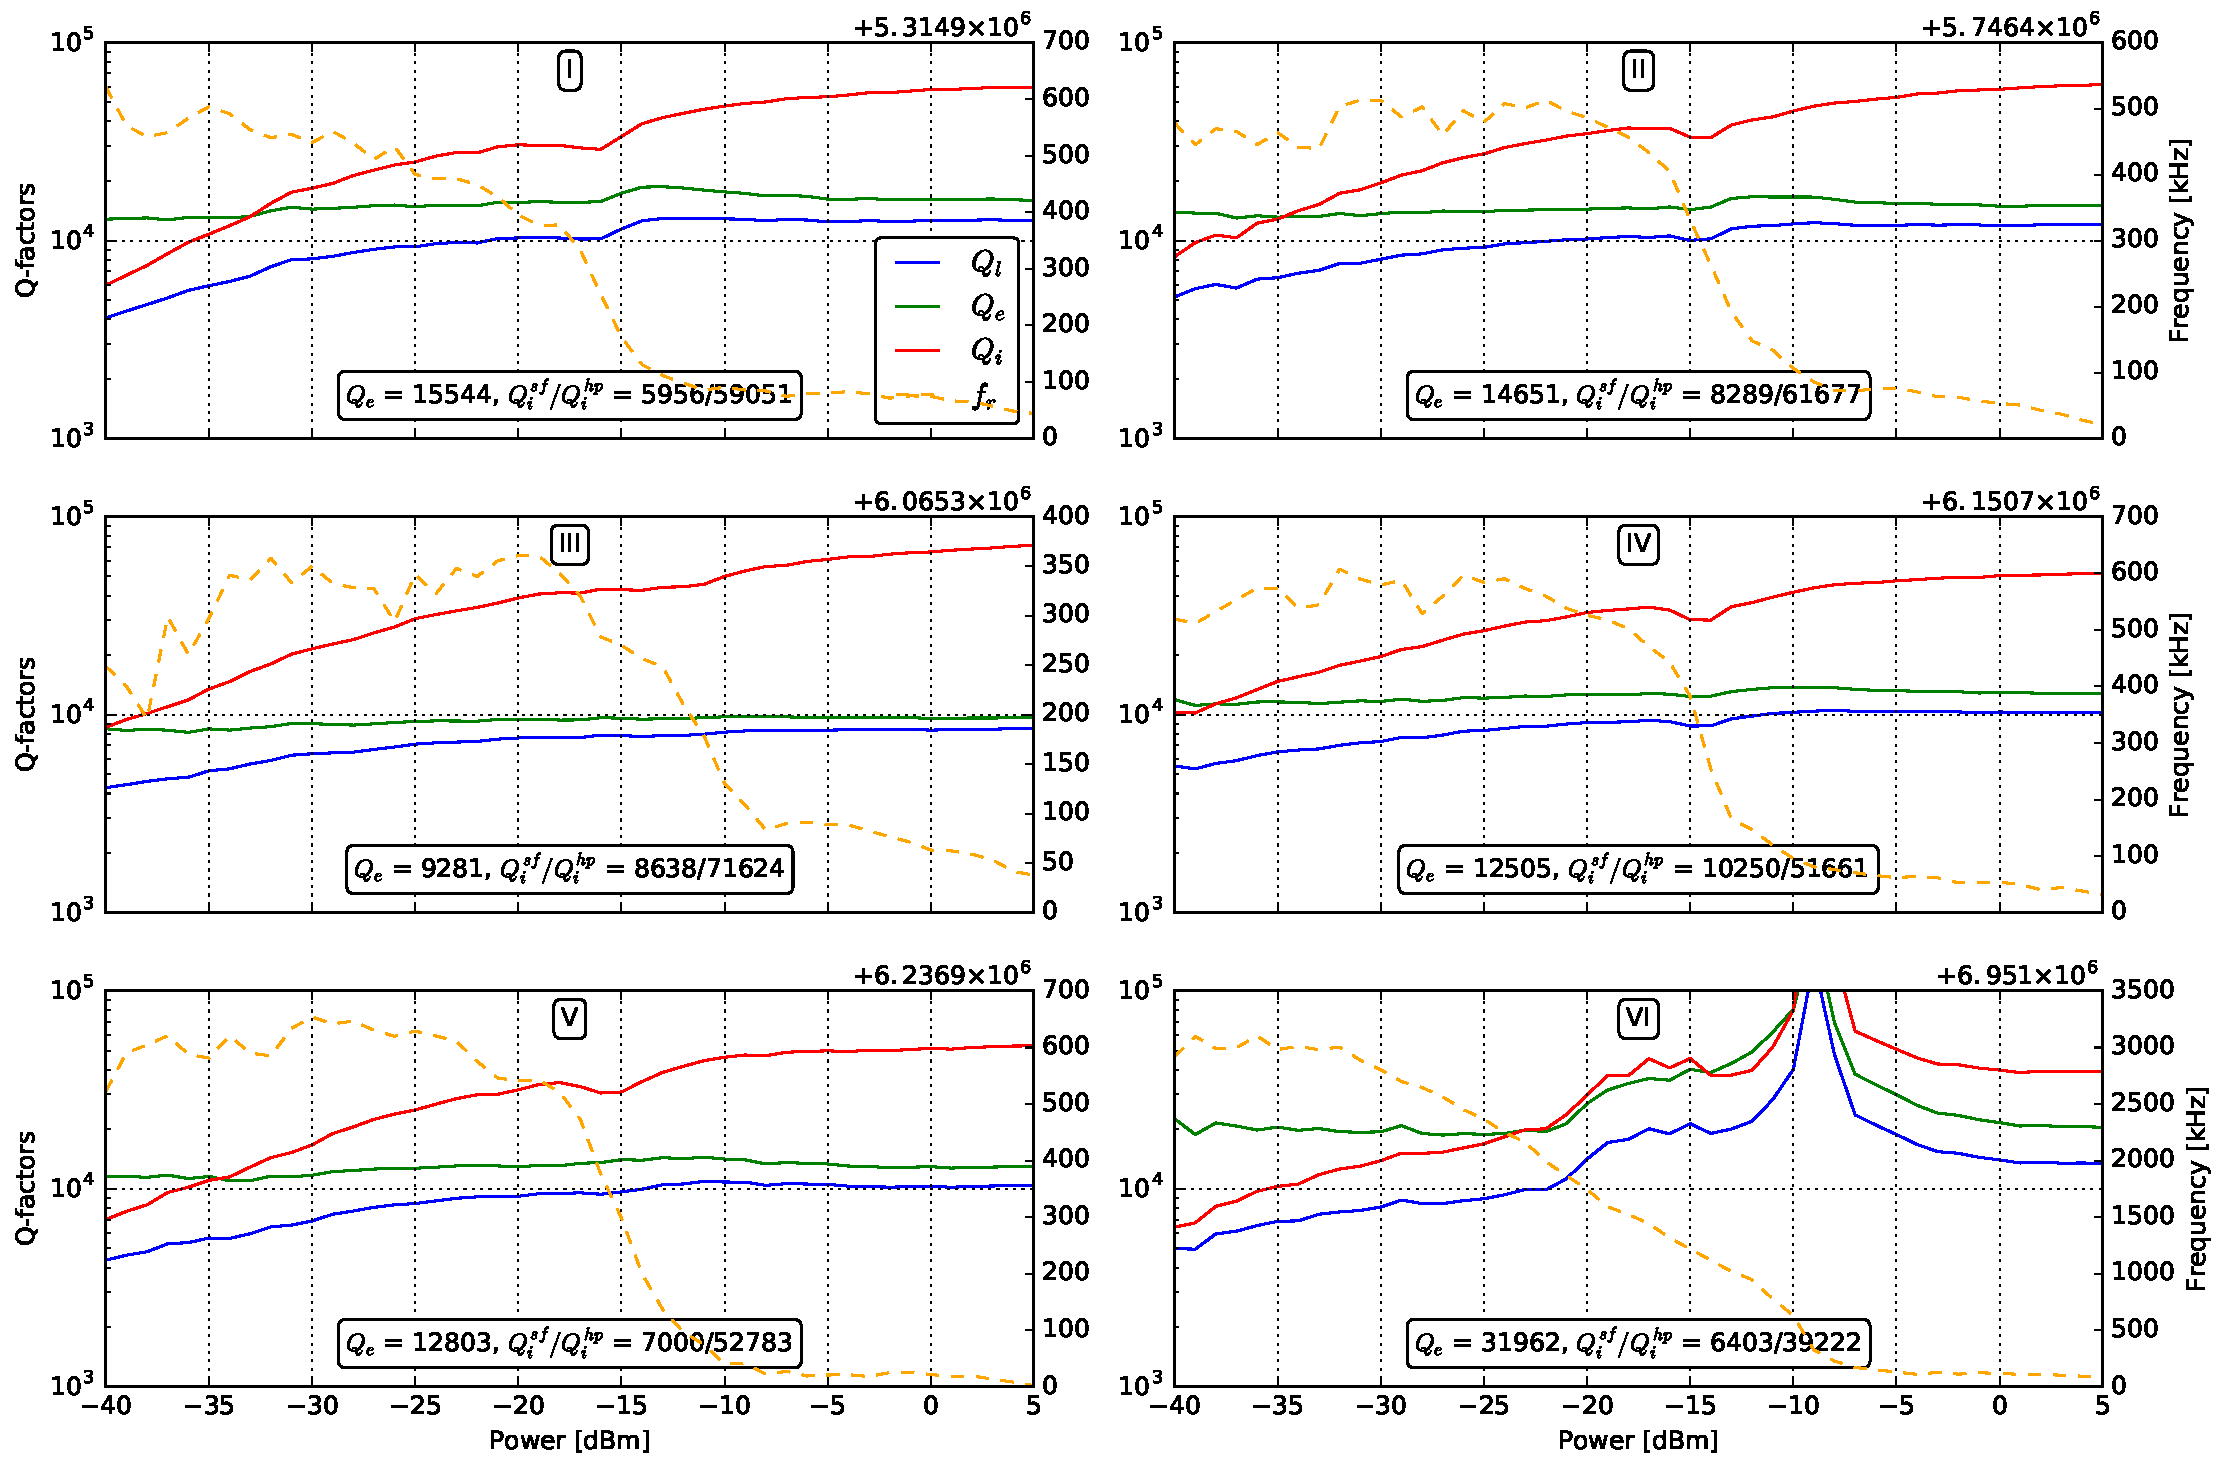
\includegraphics[width=\textwidth]{q-factors-and-freqs_xmon_first_try}
\caption{Various quality factors and frequencies depending on radiation power. Single photon limit is near -40 dBm on the VNA summed with 80 dB of attenuation, saturation limit near 5 dBm on the VNA. All devices show standard behaviour except for the VI\textsuperscript{th} which loses its shape and cannot be fit correctly at powers above -20 dBm.}
\label{fig:first_q_factors}
\end{figure}

It is well-known\cite{wang2009} that for superconducting microwave resonators the internal quality factor experiences an increase in value when probed with higher power. This effect is believed to occur due to the presence of two-level defects or two-level systems (TLS) with a dipole moment in the areas of high electric fields which resonator creates. As long as TLSs have same frequency as the measured resonator and coupled strong enough, they will drain excitations from the resonator. However TLSs can only accommodate only one photon at a time; thus, at high probe powers they saturate and do no more participate in resonator relaxation. Therefore, an increase of the internal Q-factor is observed when the resonator is driven with strong microwave fields.

When the resonator is coupled to a weakly nonlinear quantum system like transmon its quality factor will depend strongly on the coherence time of the qubit when their frequencies are close (thus on the flux bias). Therefore, possibly the low (usual $Q_i$ values for similar Al devices are around 3$\cdot 10^4$) internal quality factor values of the resonators at single-photon level are determined by high dissipation in the qubits that were not detuned far enough in frequency.

\begin{figure}
\centering
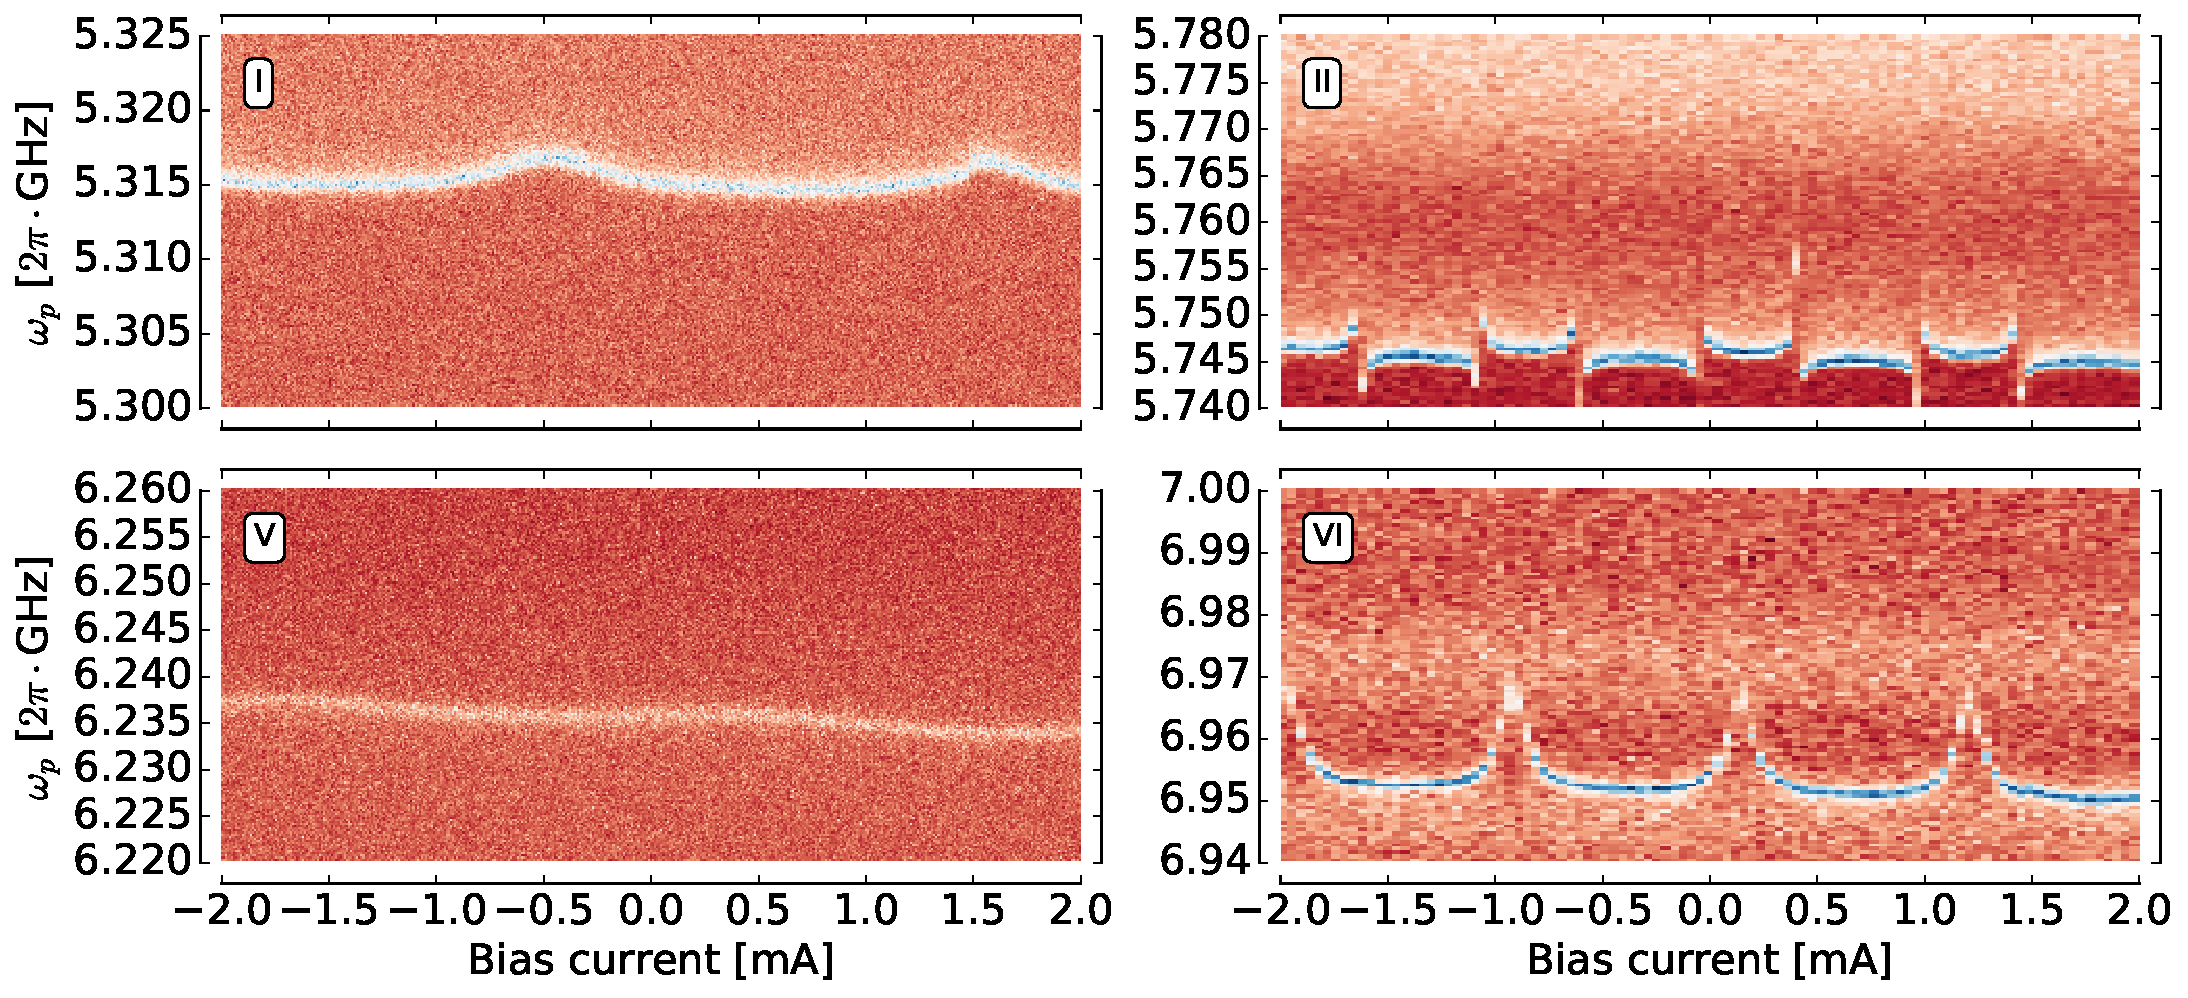
\includegraphics[width=\textwidth]{first_resonators_on_flux}
\caption{Magnetic field influence on frequencies of four devices. Resonators III and IV didn't demonstrate any significant dependence on flux (not shown here).}
\label{fig:first_resonators_on_flux}
\end{figure} 

\subsection{Characterization of the whole cQED systems}

From six systems on the chip only three were studied in detail partly due to lack of time and partly because the overall picture was more or less clear at that point. Firstly the behaviour of the resonators was investigated when the flux bias was being changed. This measurement revealed obvious periodic frequency oscillations in four devices from six, see \autoref{fig:first_resonators_on_flux}. The other two devices didn't show any noticeable periodic flux dependence because one of the qubits (III) had a broken SQUID and the other (IV) probably was much lower in frequency than its resonator.

Firstly system II was measured as long as it has shown the most prominent flux response of all. Then system VI was investigated and, finally, system I. For each of them a two-tone spectroscopy was performed and for II and VI a high-resolution single-tone one as well. Then the data was used to fit the parameters in the model \eqref{eq:hamiltonian} described in \autoref{sec:cQED}. Accordingly, the graphs that are shown below are composed of the experimental spectra overlayed with theoretical curves obtained from numerical solution of the corresponding eigenproblems.

\subsubsection{System II}

\paragraph{Model.} Below all the experimental data will be provided for system II along with theoretical fits of the spectral lines that were observed using the model \eqref{eq:hamiltonian}. Model parameters were fit based on all data on this system and are same for all figures in this section. Before turning to the comparison of the theoretical predictions and experimental results it would be useful to present the model parameters used for fitting which are summarized in \autoref{tab:first_II_params}.

\begin{table}[h]
\centering
\begin{tabular}{l|c}
Parameter & Value \\
\hline 
$C_\kappa$ & 0 fF \\
\hline
$C_g$ & 1.9 fF \\
\hline
$C_q$ & 95 fF \\
\hline
$E_C$ & 200 MHz
\end{tabular}~
\begin{tabular}{l|c}
Parameter & Value\\
\hline
$C_r$ & 444 fF \\
\hline
$L_r$ & 1.72 nH \\
\hline
$I_{C, \Sigma}$ & 69.5 nA \\
\hline
$E_{J, \Sigma}$ & 34.5 GHz
\end{tabular}
\caption{Values of the main parameters defining the spectrum of the model \eqref{eq:hamiltonian}.}
\label{tab:first_II_params}
\end{table}

From these values it's possible to calculate the coupling strength $g \approx 19.6$ MHz between the qubit and the resonator, bare qubit frequency of $\omega^{(0)}_{ge}/2\pi = 7.3$ GHz and bare resonator frequency $\omega^{(0)}_r = 5.758$ GHz. In the coupled system these values are shifted strongly, $\omega_{ge}/2\pi = 7.23$ GHz and $\omega_r = 5.746$ GHz. These shifts are so large (much greater than what would be predicted by the usual dispersive shifts) because of the large value of the Xmon capacitance. Usually cQED systems are treated in the limit of large $C_r \gg C_q, C_g, C_\kappa$ and in this case factors in the terms $\mathcal{\hat H}_q, \mathcal{\hat H}_r $ from \eqref{eq:hamiltonian} can be reduced to their bare uncoupled values. This means the only difference from the uncoupled case is the term $\mathcal{\hat H}_i$, which defines the shifts from the uncoupled frequencies, which are in this case by definition equal to the dispersive shifts. In the studied case $C_q \approx 0.25\, C_r$ and cannot be neglected; thus, the interacting systems are not the same as before coupling, and only the full model \eqref{eq:hamiltonian} taking account of all capacitances can be used to obtain correct results. Despite that after acquiring the new parameters for the interacting systems from \eqref{eq:hamiltonian} the dispersive shifts may be calculated as usual.

The flux normalization on the x-axis was done using data from \autoref{fig:first_resonators_on_flux}~(II) knowing the fact that $\Phi_0$ should be the period of the pattern and that zero flux point is situated at the center of one of the lower branches.

Below in the description of the figures a bit different notation for the transition frequencies may be used than those which denote the theoretical curves on the legends of the graphs. This is due to the fact that in the presence of coupling the qubit spectrum $\omega_{ge}(\Phi_{ext})$ is shared between transitions $\omega_{01}(\Phi_{ext})$ and $\omega_{02}(\Phi_{ext})$ of the full Hamiltonian, so when we say $\omega_{ge}(\Phi_{ext})$ we imply $\omega_{01}(\Phi_{ext})$ and $\omega_{02}(\Phi_{ext})$ for the cases of $\Delta_\omega > 0 $ and $\Delta_\omega < 0$, respectively.

\begin{figure}
\centering
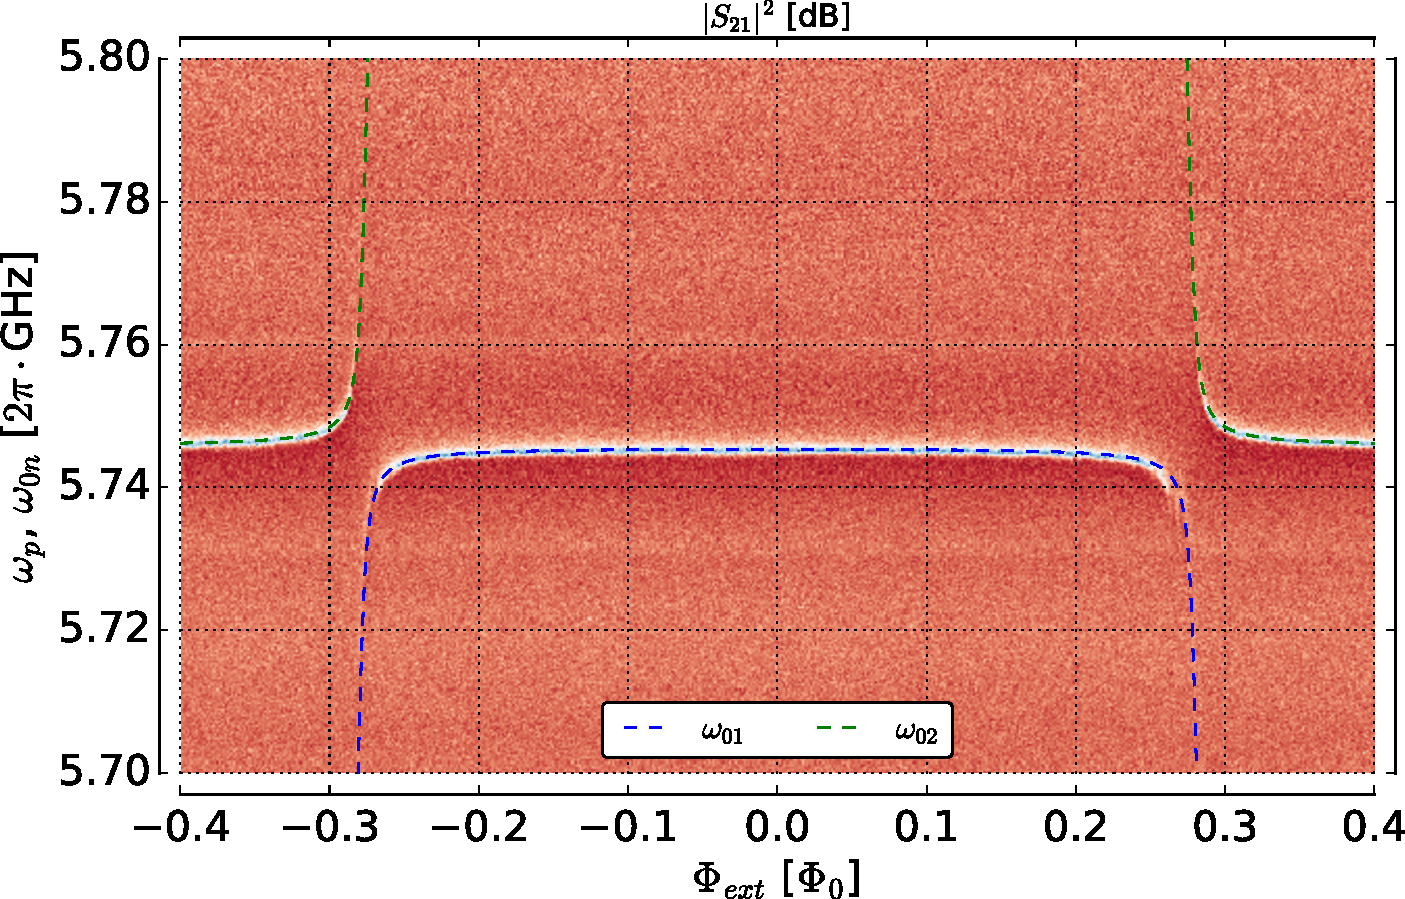
\includegraphics[width=0.9\textwidth]{first_II_anticrossing_fit}
\caption{Anticrossing spectrum of system II with fitting lines obtained by numeric calculation from the model\eqref{eq:hamiltonian} (z-axis normalized). It can be seen that lower branch has some artefacts near the anticrossings which are caused by multiphoton and sideband transitions, signifying that probe power was not at single-photon level. The x-axis is normalized to one flux quantum through the SQUID of the Xmon.}
\label{fig:first_2nd_res_anticrossing}
\end{figure} 

\paragraph{Anticrossing spectrum.} Firstly, a high-resolution scan of one of the anticrossings from \autoref{fig:first_resonators_on_flux}~(II) was obtained. The power level on the VNA was set to -40.0 dBm, which means around -120 dBm at the sample. It is presented in \autoref{fig:first_2nd_res_anticrossing}. It can be seen that a really good agreement between experiment and theory was attained. However there are some discrepancies that can be pointed out: a slight asymmetry of the left and right anticrossings and the reduced brightness of the main branch $\omega_{01}$ on the right. It can be seen clearly from the data that additional multi-photon transitions or sidebands are visible similar to what have been observed before\cite{bishop2009} which indicates that the power was higher than at the single-photon level. Theoretical curves for those transitions were not displayed because the picture becomes too crowded. It is not clear why this effect is stronger in the right anticrossing than in the left one. Further investigation is needed, because at that cooldown due to the setup limitations measurements at lower power were too time consuming because of the low transmission.

\begin{figure}
\centering
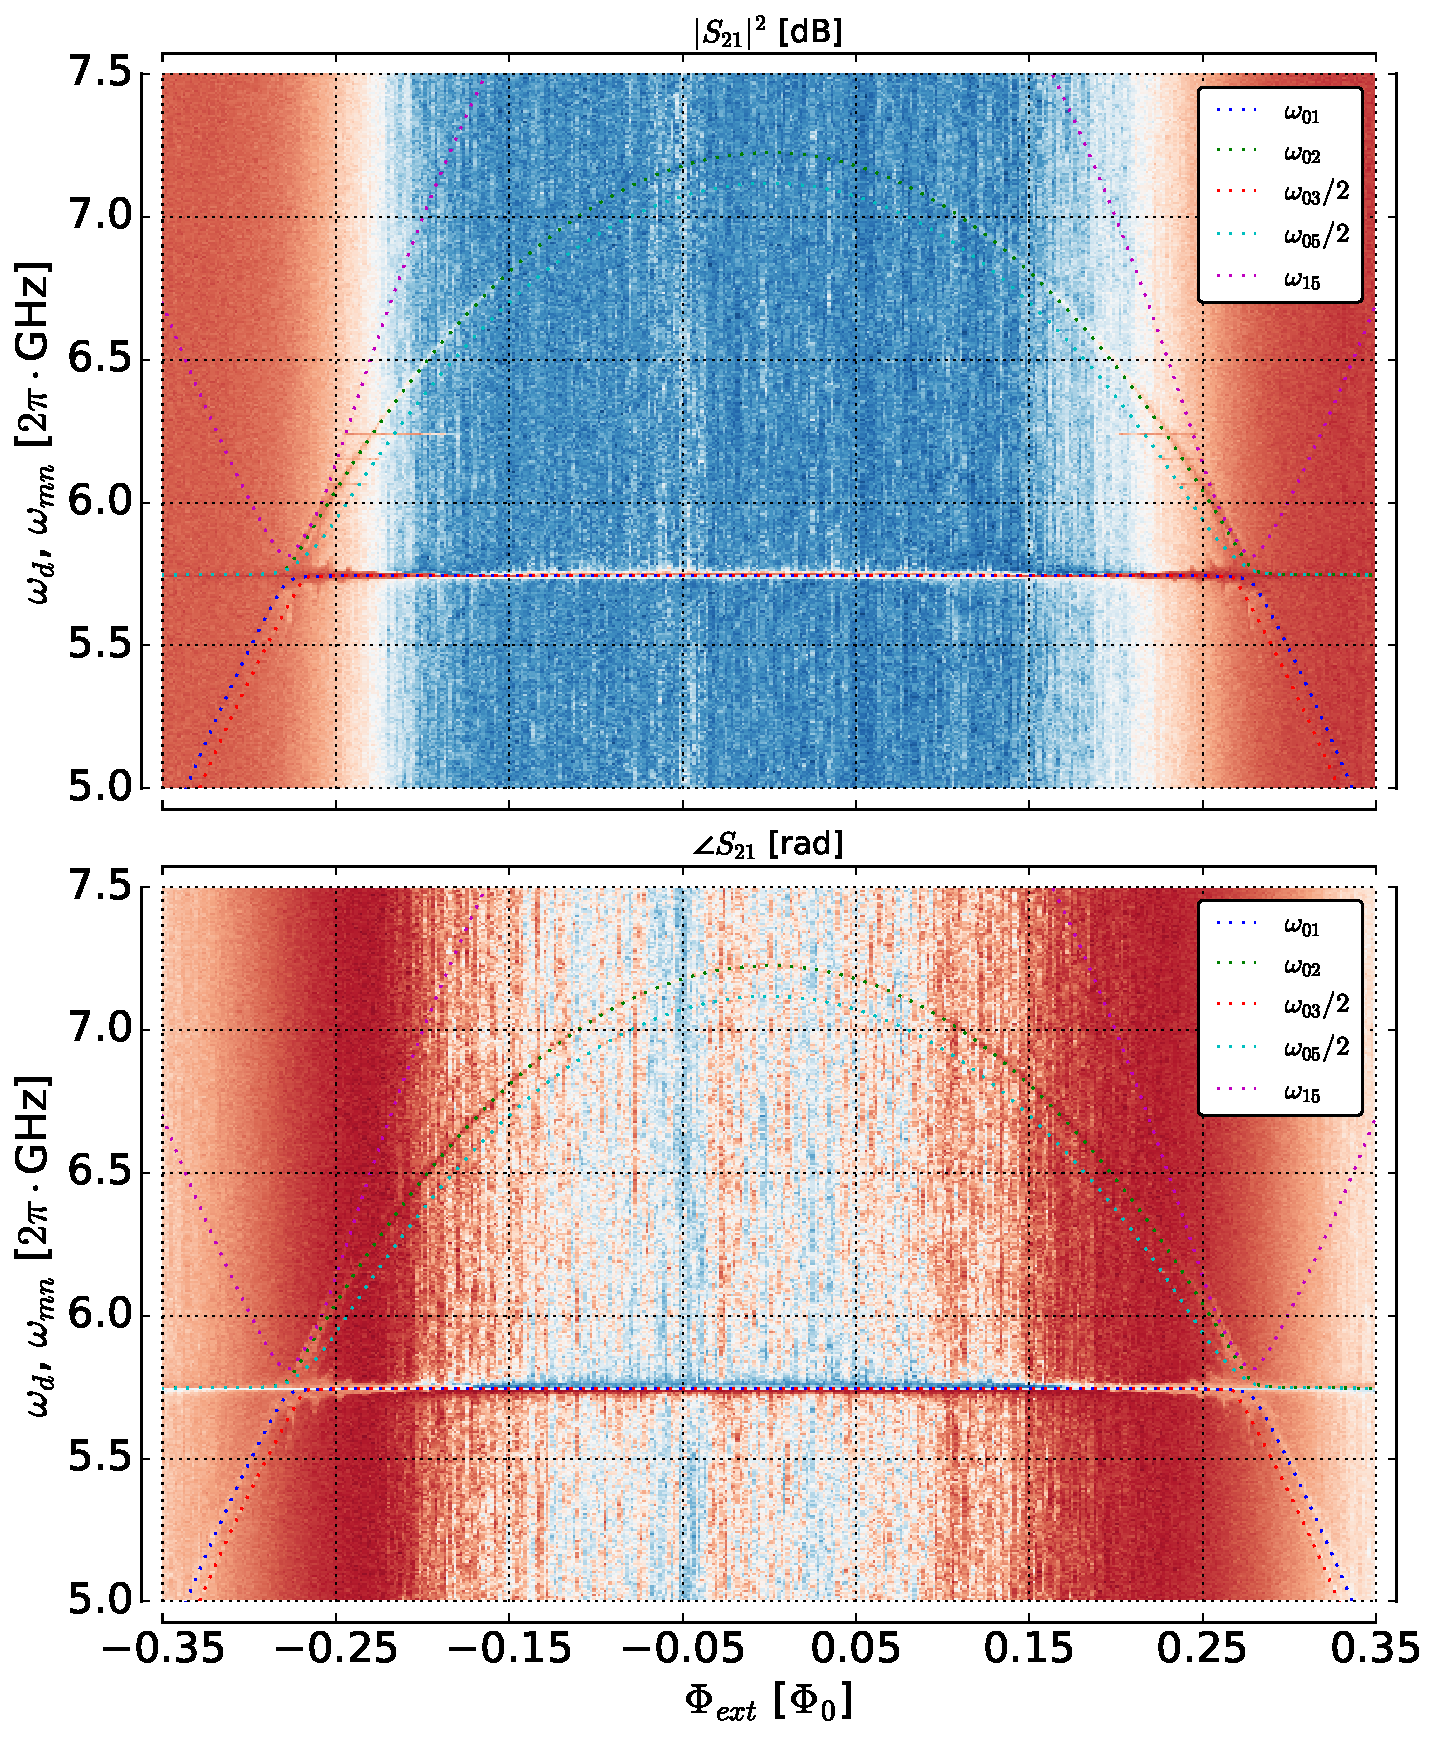
\includegraphics[width=.9\textwidth]{first_II_2tone_fit}
\caption{The two-tone spectrum of system II at -20 dBm power level on the $\mu$-wave source with fitting lines obtained from the model \eqref{eq:hamiltonian}. Various transitions are visible, most pronounced are the horizontal resonator $0n$ transition, the hyperbolic qubit $ge$ transition ($\omega_{01},\ \omega_{02}$) and lower branch of the hyperbolic two-photon $gf$ transition ($\omega_{03}/2$). Also a sideband $\ket{1,g}\rightarrow \ket{0,f}$ is visible ($\omega_{15}$).}
\label{fig:first_II_2tone}
\end{figure}


\paragraph{Two-tone spectroscopy.} Next measurement was a standard two-tone spectroscopy. The results of such measurement at different second tone powers are presented. Firstly, the lowest possible power (-20 dBm) scan was acquired, it is shown in \autoref{fig:first_II_2tone}. It was not possible to set a lower power with the step attenuator of the $\mu$-wave source, however for studied system that power was low enough to observe only single-photon processes without apparent multi-photon transitions and sidebands around the qubit's degeneracy point. However due to the fact that the second tone was introduced from the feedline through the resonator the effective driving power was increasing when the qubit-resonator detuning was decreasing; thus, some secondary transitions become visible near the anticrossing regions. For example, a sideband transition which uses one photon from a resonator and one photon from the incident microwave radiation ($\omega_{15}$) is vaguely visible above the resonator line and a two-photon transition $\omega_{gf}/2$ is clearly visible below it.

\begin{figure}
\centering
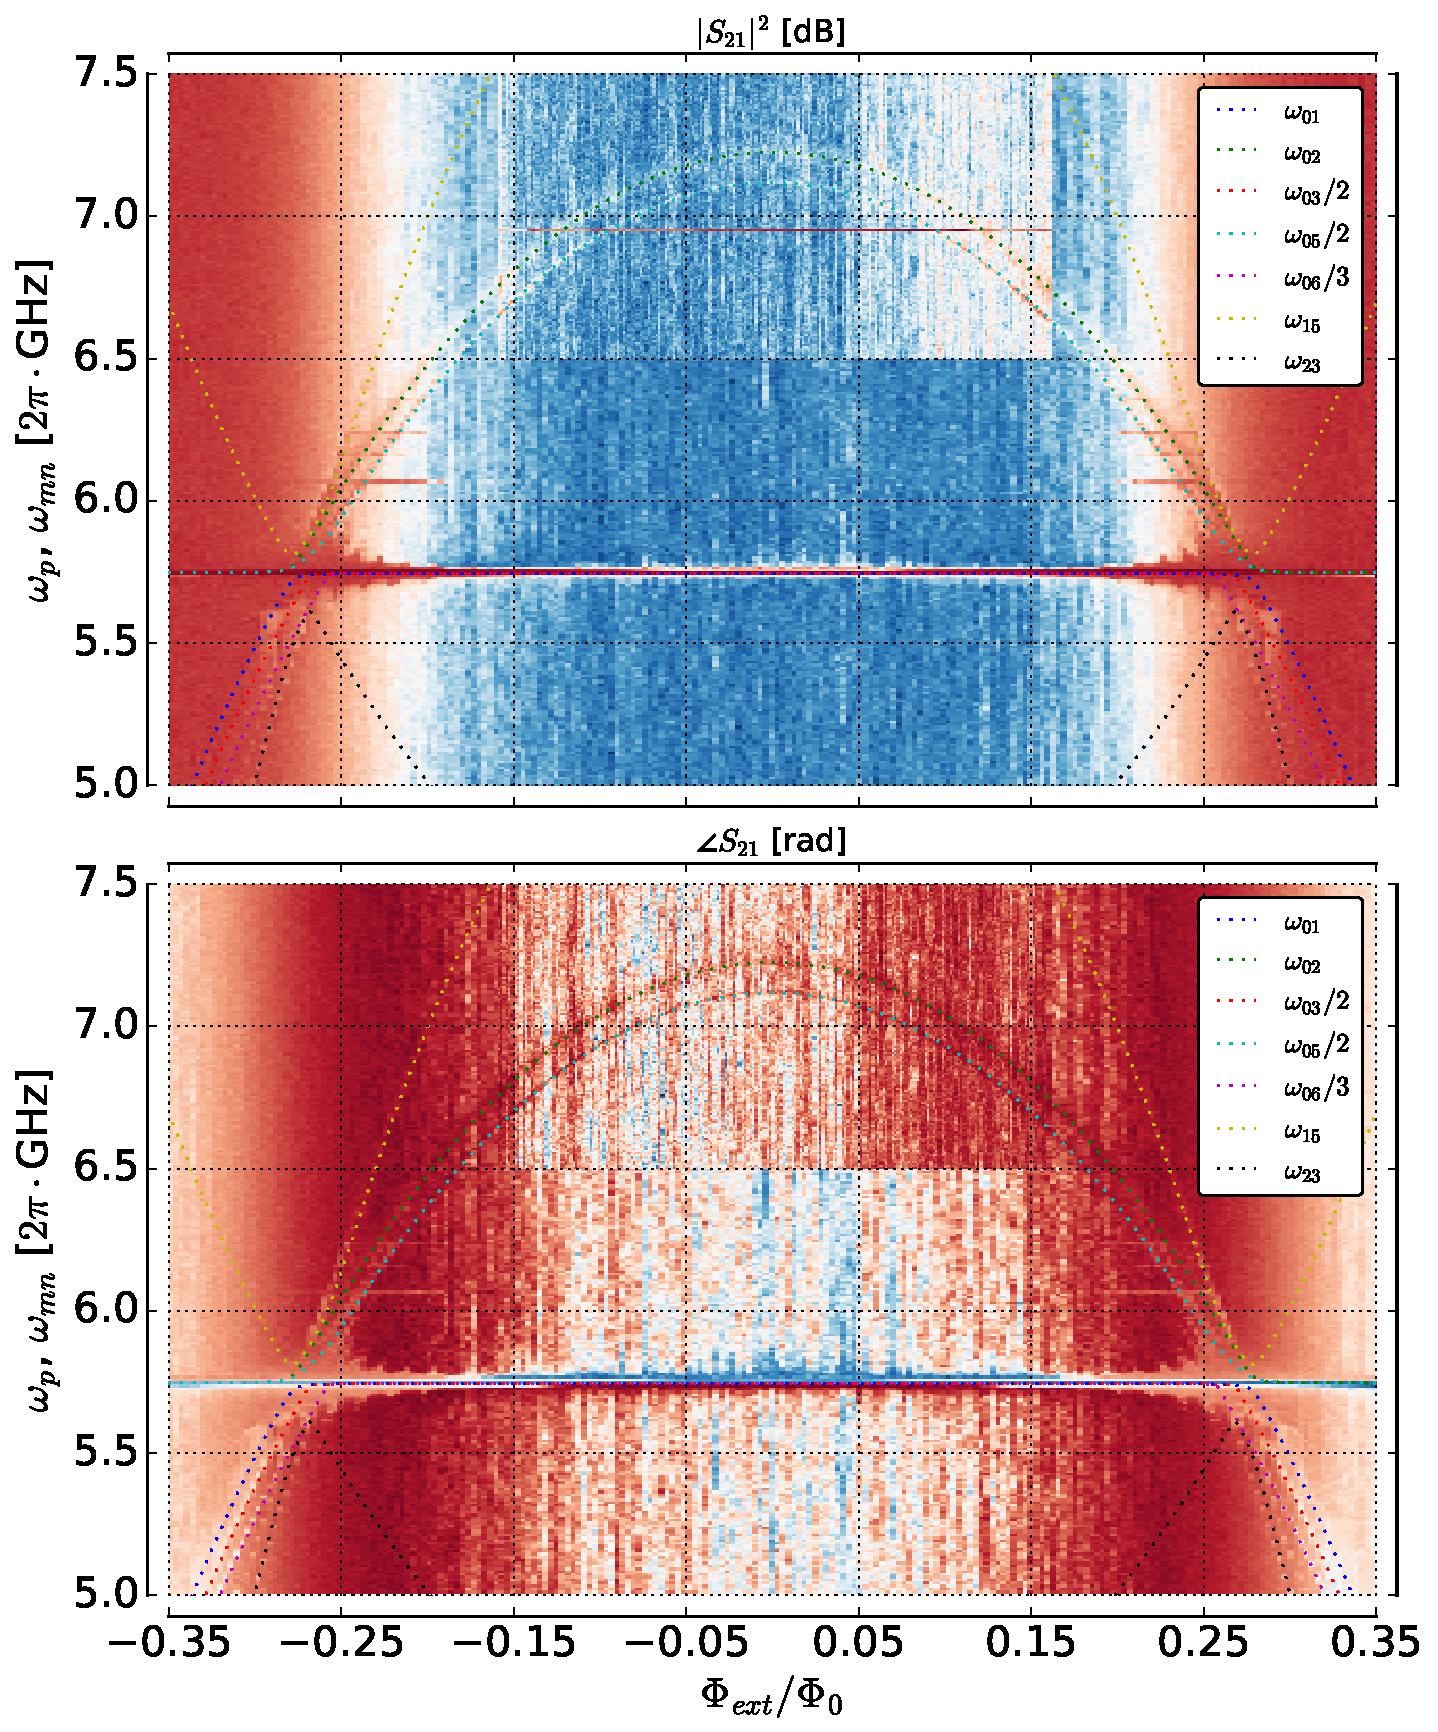
\includegraphics[width=.9\textwidth]{first_II_2tone_higher_power_fit}
\caption{The two-tone spectrum of system II at -10 dBm power level on the $\mu$-wave source with fitting lines obtained from the model \eqref{eq:hamiltonian}. More transitions are visible, new compared to \autoref{fig:first_II_2tone} are the upper branch of the two-photon $gf$ transition ($\omega_{05}/2$), the lower branch of the three-photon $gd$ transition ($\omega_{06}/3$) and also the lower branch of the sideband $\ket{1,g}\rightarrow \ket{0,f}$ ($\omega_{23}$).}
\label{fig:first_II_2tone_hp}
\end{figure}

If the power of the second tone is increased, the probability of the transitions with lesser matrix elements also rises allowing to see these transitions more clearly. Such measurement yields a spectrum as in \autoref{fig:first_II_2tone_hp}. It was done at -10 dBm; thus, a power 10 times higher than in the previous case was sent at the sample. Now the two-photon hyperbolic line $\omega_{gf}$ under the main one $\omega_{ge}$ is clearly visible (the upper complementary branch $\omega_{05}/2$ of the previously visible transition $\omega_{03}/2$). The upper branch of the sideband $\ket{1,g}\rightarrow \ket{0,f}$ is visible also, see \autoref{fig:first_II_2tone_zoom_fit} for the scan around $\Phi_{ext}=0$. Also there are two lines below the resonator at the sides of the graph whose origin is not clear. One of them might be the lower branch of that sideband (fit with $\omega_{23}$ in \autoref{fig:first_II_2tone_hp}), however it can be seen that the theoretical line is not very accurate there. The other line which is visible between $\omega_{23}$ and $\omega_{06}/3$ was not fit because no appropriate transition was found. Surely, one should be able to find it but this task looks hard enough to give it up.

	
\begin{figure}
\centering
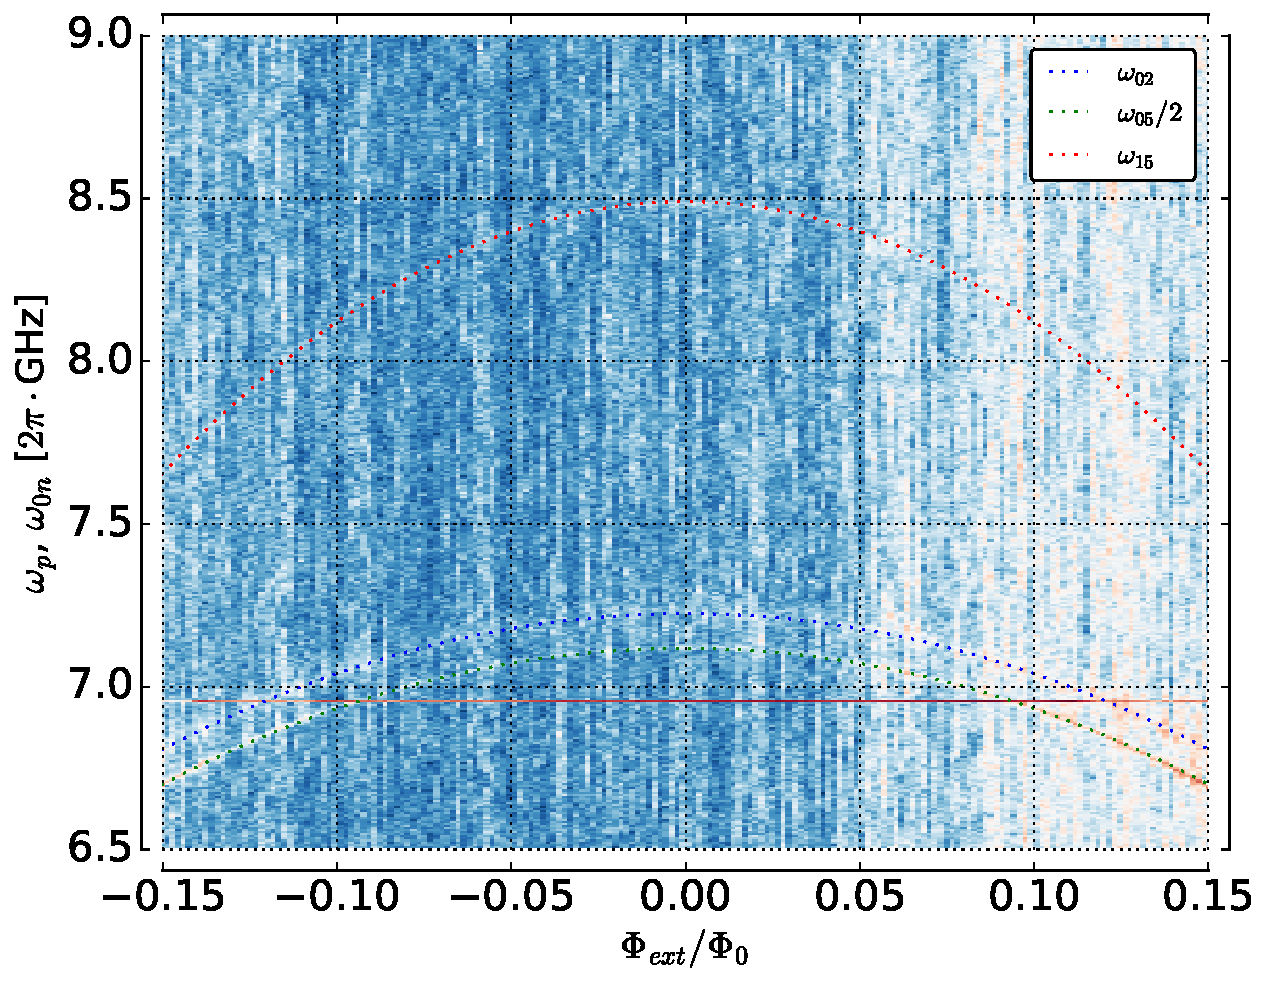
\includegraphics[width=0.8\textwidth]{first_II_2tone_zoom_fit}
\caption{Zoomed area around the main qubit transition $ge$, two-photon transition $gf$ and the sideband transition $\ket{1,g}\rightarrow \ket{0,f}$ with fitting lines. Second tone power was -10 dBm, transmission amplitude is displayed.}
\label{fig:first_II_2tone_zoom_fit}
\end{figure}

Interestingly enough as well as the transition corresponding to the system's resonator some other narrow horizontal transitions are visible. Three of these lines are visible best of all around 6.1 GHz near the qubit line in \autoref{fig:first_II_2tone}~($|S^2_{21}|$) and near 7 GHz in the high-resolution area of \autoref{fig:first_II_2tone_hp}~($|S^2_{21}|$). They correspond to the other resonators which lie higher in frequency. This effect was already observed before but was not thoroughly studied. At this moment it seems that the effect of changed transmission on the probe frequency when the other resonator is resonantly excited with large power (second tone power is 10$^4$-10$^5$ times higher than the probe power) is not due to the coupling of the resonators but due to nonlinear effects or suppressed superconductivity in the Al film itself.

\newpage

\subsubsection{System VI}

\paragraph{Model.} Below all the experimental data will be provided for system VI along with theoretical fits of the spectral lines that were observed using the model \eqref{eq:hamiltonian}. Model parameters were fit based on all data on this system and are same for all figures in this section. Before turning to the comparison of the theoretical predictions and experimental results it would be useful to present the model parameters used for fitting which are summarized in \autoref{tab:first_VI_params}.

\begin{table}[h]
\centering
\begin{tabular}{l|c}
Parameter & Value \\
\hline 
$C_\kappa$ & 0 fF \\
\hline
$C_g$ & 1.8 fF \\
\hline
$C_q$ & 95 fF \\
\hline
$E_C$ & 200 MHz
\end{tabular}~
\begin{tabular}{l|c}
Parameter & Value\\
\hline
$C_r$ & 367 fF \\
\hline
$L_r$ & 1.41 nH \\
\hline
$I_{C, \Sigma}$ & 63.4 nA \\
\hline
$E_{J, \Sigma}$ & 31.5 GHz
\end{tabular}
\caption{Values of the main parameters defining the spectrum of the model \eqref{eq:hamiltonian}.}
\label{tab:first_VI_params}
\end{table}

\paragraph{Anticrossing.} The anticrossing spectrum of the sixth system is presented in \autoref{fig:first_VI_anticrossing_fit}. It can be directly seen that the qubit is very close in frequency to its resonator; thus, the resonator line is bent slightly and the qubit line is looking ordinary. Using the theoretical model \eqref{eq:hamiltonian} these two lines were fit, and there's a good agreement between theory and data. It can be seen that at the degeneracy point, where the qubit is closest in frequency to the resonator, the resonator line becomes dimmer; it indicates that the qubit is less coherent than the resonator, reducing its Q-factor when approaching resonant interaction.

\begin{figure}
\centering
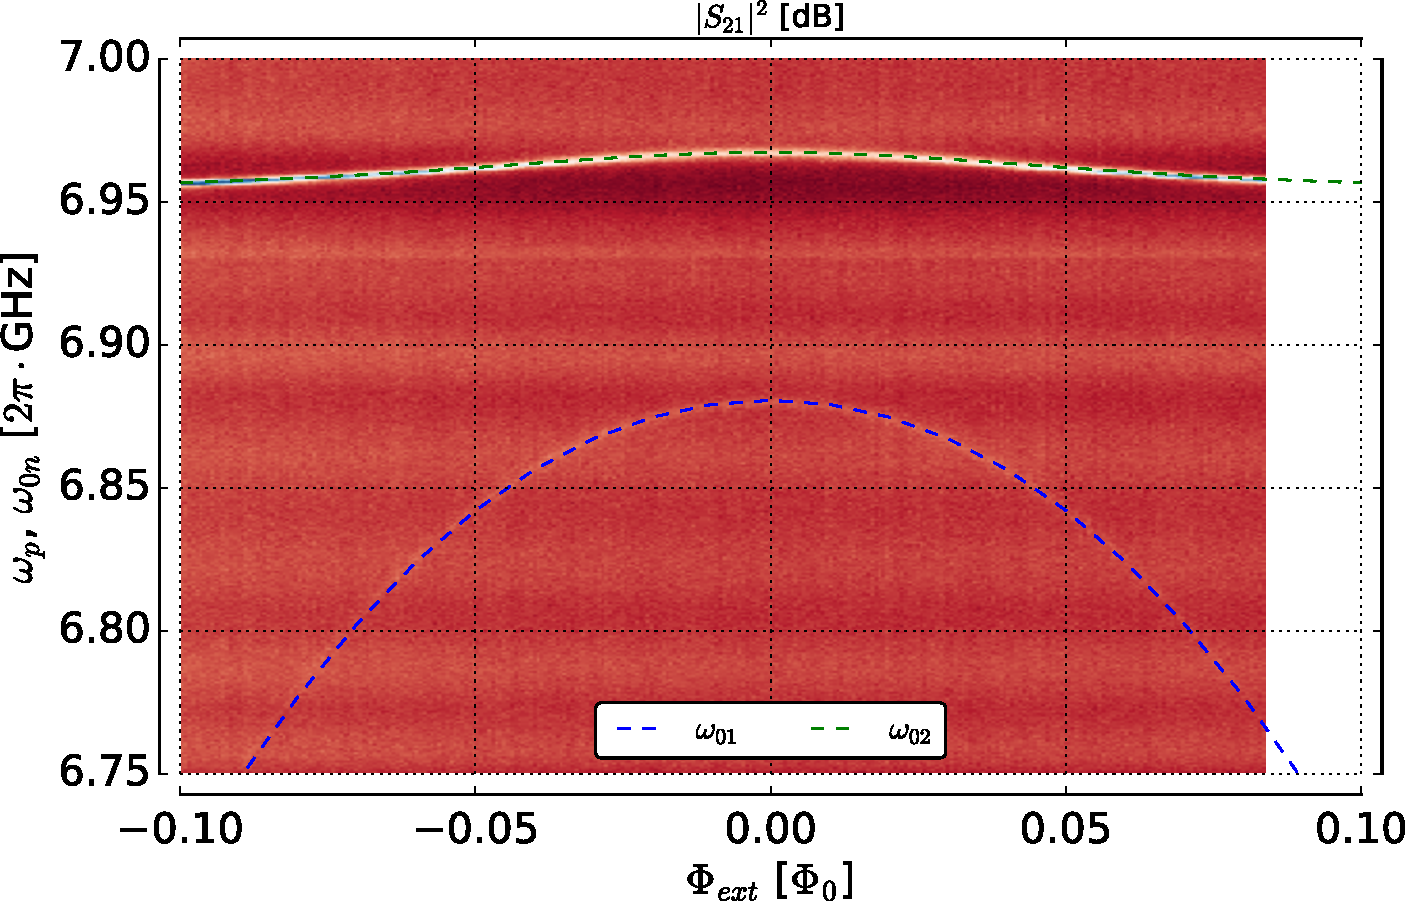
\includegraphics[width=0.9\textwidth]{first_VI_anticrossing_fit}
\caption{Anticrossing spectrum for the 6$^\text{th}$ system (z-axis normalized) with fitting lines obtained from the model \eqref{eq:hamiltonian}. }
\label{fig:first_VI_anticrossing_fit}
\end{figure}

\paragraph{Two-tone spectroscopy.} The results of the two-tone spectroscopy are presented in \autoref{fig:first_VI_2tone_fit}. It was performed at the lowest possible power of -20 dBm on the $\mu$-wave source, yet, due to a very small detuning of the qubit at the degeneracy point, the power in

\begin{figure}
\centering
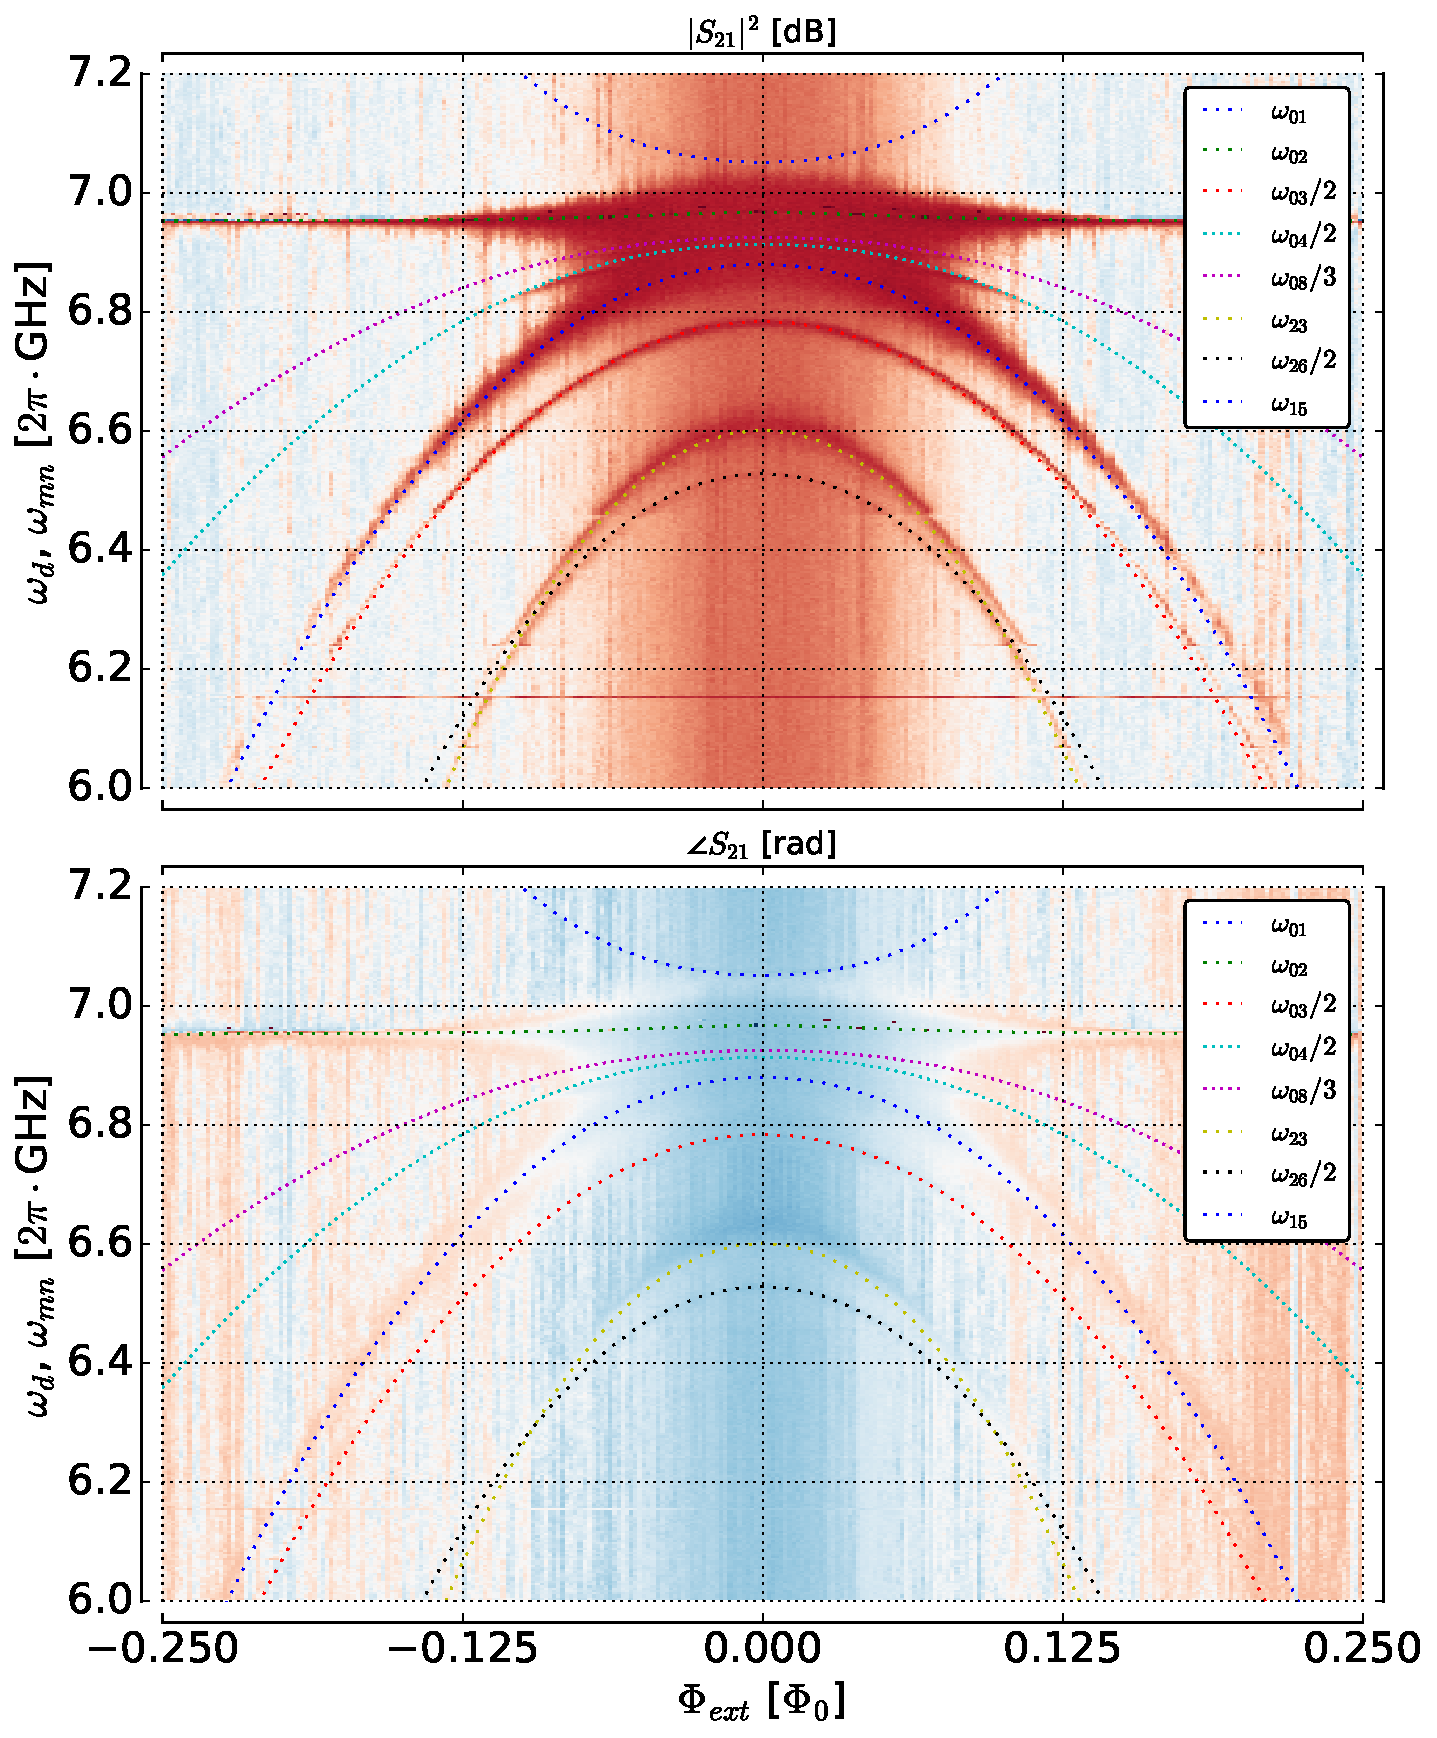
\includegraphics[width=.9\textwidth]{first_VI_2tone_fit}
\caption{Two-tone spectrum of the 6$^\text{th}$ system (z-axis normalized) at -20 dBm on the $\mu$-wave source with fitting lines obtained from the model \eqref{eq:hamiltonian}. As long as the qubit is very close to the resonator in frequency the effective driving power on it is very high, and thus a lot of sideband and multiphoton transitions are visible.}
\label{fig:first_VI_2tone_fit}
\end{figure}

\newpage

\section{On-chip control lines testing design}

\subsection{Geometry and parameters}

The second design that was developed was intended to test the properties of the control lines, i.e. flux bias lines and microwave driving lines, implemented on the chip. The design is presented in \autoref{fig:second_design_full} where some of its key features are highlighted. It's 10x5 mm.

\begin{figure}[h!]
\centering
\includegraphics[width=0.7\textwidth]{chip_design2}
\includegraphics[width=0.7\textwidth]{chip_design2_zoom}
\caption{\textbf{(a)} Large-scale image of the lines testing design. The chip (8x4 mm) consists of eight $\lambda/4$ CPW resonators coupled capacitively to the feedline, six low-Q$_e$ with Xmon qubits at the open end and two high-Q$_e$ with no qubits. \textbf{(b)} Zoomed area around one of the qubits, showing the microwave antenna configuration. \textbf{(c)} Zoomed area around another qubit, showing the flux bias line. \textbf{(d)} Zoom around one of the qubits' SQUIDs. Pink areas denote the part of the mask which produces the SQUID and should be patterned with higher resolution.}
\label{fig:second_design_full}
\end{figure}

Firstly, differently from the previous design, this design has more resonators, additional two (TI, TII, see \autoref{fig:second_design_full}(a)) were inserted at the ends of the main resonator-qubit array (I-VI). These resonators have high Q$_e$ from their geometry to yield accurate results for possible high internal Q-factors.

Secondly, the frequencies of the devices were changed. The qubits still are all calculated to have the same frequency, but it's now 6 GHz, with $C_\Sigma \approx 80$ fF and $I_{C, \Sigma} = 40$ nA. The size of each junction in the qubit's SQUID is 100x200 nm$^2$. The resonators had frequencies of 7, 7.1, 7.2, 7.3, 7.4, 7.5 GHz for the cQED systems I-VI, and the bare resonators TI and TII had 8 and 8.25 GHz, respectively.

Finally, as the main change made to the design, some coplanar control lines were introduced. For the upper qubits they are microwave antennas, i.e. open-ended coplanar line pieces, to induce transitions while for the lower qubits they are flux-bias lines to change the energy level structure of the devices. The lines were separated in such a way to make the design more fault-tolerant.

Four test structures at the sides of the chip were also included to allow direct DC measurement of the SQUIDs created during the shadow evaporation.


\begin{figure}
\centering
\includegraphics[width=0.6\textwidth]{xmon_al_bmstu_1_in_pcb}
\caption{Bonded Xmon Al BMSTU 1 in the PCB of the sample holder, as seen through the microscope of the bonding machine.}
\label{fig:first_tight_fit}
\end{figure}

\subsection{Implementation and purposes}

The chip Xmon Al BMSTU 1 was made in a single-step process. It had a mask patterned with e-beam in the cleanroom facility at Bauman Moscow State Technical University (add recipe?), and then Al film was shadow-evaporated on Plassys in the RQC lab in ISSP, 25 and 45 nm thick. The substrate used was made of high-resistivity Si ($> 6$ kOhm/cm).

One significant difference about this sample is that in fact it was fabricated with its twin in the center of a larger substrate (15x15 mm) which was previously patterned on the back side with a circular saw to allow the substrate to be cracked around the chips precisely. However, the process wasn't yet mastered, and the twin chip was lost during the separation. But nevertheless, the remaining sample fitted in the PCB cutout really well (see \autoref{fig:first_tight_fit}), and the method will be further improved.


Purposes for the design:
\begin{enumerate}[label=(\alph*), leftmargin=1.5cm]
\itemsep0pt
\item to test resonator Q without qubits

\item to test lines

\item to test again the qubits' basic parameters

\item to test improvement of the noise

\item to test the half-sawing of the sample with following cracking
\end{enumerate}

\subsection{Measurement setup  STUBBED from first chip, needs review}

The sample was measured at ISSP in laboratory of RQC. Cryogenic equipment was represented by BlueFors LD250 dilution refrigerator, with base temperature of 16 mK. The microwave equipment included R\&S ZNB 10 kHz-20 GHz vector network analyser,  Agilent E8257D 100 kHz - 40 GHz analog signal generator. The sample was flux biased using Keithley 6221 current source.

Microwave line was thermalized with 60 dB of attenuation, additional 20 dB of attenuation were introduced on a directional coupler which added the second tone from the $\mu$-wave source. After leaving the sample the signal passed through two isolators and a hybrid coupler, which was used before to measure two samples during single cooldown. Finally, the signal was amplified with 4-8 GHz LNF amplifier at 4 K and a with a room-temperature amplifier.

The sample holder that was used was designed for 10x10 mm chips, so the bondwires had a relatively large length of 1 mm which of course deteriorated the overall transmission. Chip lay directly on the copper disk of the bottom part of the sample holder with no hole carved under it. Around the sample holder a superconducting coil was wound which has been supplied using the current source mentioned above.

The magnetic shielding of the sample holder was achieved via a cryoperm shield. A superconducting shield was not installed in this run due to the lack of space inside the magnetic shield, which may have influenced the noise background.

\begin{figure}[h!]
\centering
\includegraphics[width=0.9\textwidth]{xmon_al_bmstu_1_general}

\includegraphics[width=0.9\textwidth]{xmon_al_bmstu_1(2)_general}

\includegraphics[width=0.9\textwidth]{xmon_al_bmstu_1(3)_general}


\caption{\textbf{(Top)} General view of the resonances. All six resonances are visible, however shifted down in frequency. This shift more or less consistent throughout the devices, and thus it's most probably caused by effective $\epsilon_{Si}$ different from the one used in the calculation. \textbf{(Middle)} General view of the resonances (2$^\text{nd}$ cooldown). Transmission now lower as a 5 dB attenuator was replaced by a 10 dB one. Seven resonances are visible, as the second resonator presumably coupled to something. The shapes of the other peaks also changed. \textbf{(Bottom)} General view of the resonances (3$^\text{d}$ cooldown).  Transmission is 20 dB higher as the directional coupler was altered. Again, six resonances are visible, though some spurious dip is present between devices III and IV, and the shapes changed again.}
\label{fig:second_resonators_general}
\end{figure}


\begin{figure}[h!]
\centering

\includegraphics[width=\textwidth]{q-factors-and-freqs_xmon_al_bmstu_1}

\caption{Various quality factors and frequencies depending on radiation power. Some resonators show interesting dip in internal Q near -25 dBm and significant change in frequency, implying they are coupled to functioning qubits saturation of which causes the effect. Other resonators do not show such features.}
\label{fig:second_q_factors}
\end{figure}

\begin{figure}[h!]
\centering
\includegraphics[width=\textwidth]{q-factors-and-freqs_xmon_al_bmstu_1(2)}
\caption{Same figure for the 2$^\text{nd}$ cooldown. Significant deviations are present in comparison with the first cooldown, both to the greater and to the lower Q-factors on different devices.}
\label{fig:second_q_factors(2)}
\end{figure}

\begin{figure}[h!]
\centering
\includegraphics[width=\textwidth]{q-factors-and-freqs_xmon_al_bmstu_1(3)}
\caption{Same figure for the 3$^\text{d}$ cooldown. The Q-factors degraded completely both for the cQED resonators and the test resonators.}
\label{fig:second_q_factors(3)}
\end{figure}

\subsection{Characterization of the resonators}

The resonators on the sample were measured several times (after each new cooldown) as they seemed to degrade. Indeed, looking at the Q-factors over the cooldowns reveals that the resonators got worse and worse, even if nothing at all was done with the chip.

Before the second cooldown the chip was moved out of the PCB to solder additional SMP connectors on it, and then moved back in. No mechanical damage or contamination was inflicted to it. However, we can see dramatic changes in quality factors of the resonators, some got better and some got worse for unknown reasons (see \autoref{fig:second_q_factors(2)}). Devices II and III got so bad it was impossible to fit them as their widths compare to the S$_{12}$ general roughness features (see \autoref{fig:second_resonators_general} (Top) vs (Middle)).

After that before the third cooldown nothing at all was done to the chip. After the cooldown and before the Q-factor measurement there was an accidental excessive current through the surrounding coil. Though, it didn't change the general appearance of the resonances which was again found different at this cooldown (see \autoref{fig:second_resonators_general} (Bottom)). At this run the Q-factors became unacceptably low (see \autoref{fig:second_q_factors(3)}) at all powers. 


\subsection{Characterization of the cQED systems}

The two systems were possible to study in this sample, I and VI. Others either did not indicate presence of the functional qubits or experience strong flux hopping while tuned via the superconducting coil and don't have the flux bias lines attached to work around this problem. Fortunately, system I has the qubit with the flux bias line and system VI has the microwave antenna, so both these on-chip devices were successfully tested.



\subsubsection{System I}

The system one was biased by the superconducting loop right on the chip. This allows to make wide scans without affecting negatively the resonator with the width limited only by the current source. The periodic spectrum of the anticrossings for system I is displayed in \autoref{fig:second_I_anti}. The pattern is shifted noticeably to the left due to some residual field around the sample.

\begin{figure}[h]
\centering
\includegraphics[width=\textwidth]{second-I-anti}
\caption{Periodic anticrossing picture for the system I (at high power). The current on the current source spans 80 mA and is actually comparable at the endpoints to it's maximum possible output of 105 mA.}
\label{fig:second_I_anti}
\end{figure}

\begin{figure}[h]
\centering
\includegraphics[width=\textwidth]{second-I-spec-lines}

\includegraphics[width=\textwidth]{ge-linewidth}
\caption{Qubit spectrum at 0 dBm on the output of the 2$^{\text{nd}}$ tone generator (left), dependence of the linewidth on the driving power (right) and high-resolution scan of the two-tone peak at -20 dBm (bottom).}
\label{fig:second_I_spec_lines}
\end{figure}


The experiment to determine qubit spectrum and the linewidth at the degeneracy point was also done on the system. The resulting graphs are presented in \autoref{fig:second_I_spec_lines}. On the right plot the spectrum of the qubit is visible; it consists of three lines corresponding to the transitions $ge,\ gf/2$ and $gd/3$ and visible due to the high power of the drive. On the left plot the spectral line width is recorded over the incident power of the drive. It's possible to estimate the linewidth of the bare qubit from the phase 2-tone data (see Section \ref{sec:2tone}). The line experiences significant broadening with increased power; though, at the minimal possible power of -20 dBm it's width is very small, around 0.5 MHz, which allows to set a lower bound of 300 ns on the qubit $T_1$ (assuming that there's no pure dephasing due to the flux fluctuations at the sweet spot and to the excessive population of the resonator as $\delta\omega = \frac{1}{T_1}+\frac{2}{T_2}$).

\subsubsection{System VI}

System VI had an on-chip microwave antenna nearby, but had no flux bias line (see \autoref{fig:second_design_full}), and thus had to be biased by the external coil. With the studied sample this method of biasing was very inconvenient, as even small magnetic field from the coil influenced the resonators tremendously, inducing continuous and discontinuous frequency shifts in them, presumably due to flux creep and hopping. Fortunately, is was still possible to tune the qubit of the VI$^{\text{th}}$ system enough to observe it's spectrum and to test the microwave antenna.

\begin{figure}
\centering
\includegraphics[width=0.7\textwidth]{second_VI_anti}
\caption{Anticrossing of the VI$^{\text{th}}$ cQED system. It can be seen that the picture is not symmetric and   the lines are bent downwards at the ends, as the resonator frequency change was caused not only by the qubit, but also directly by the magnetic field.}
\label{fig:second_VI_anti}
\end{figure}

The anticrossing measured for this system is shown in \autoref{fig:second_VI_anti}. It was hard to measure, though, as the flux hopping was interfering with the tuning of the qubit. The resonator frequency change due to the magnetic field has bent the picture, so it would be impossible to fit it within the model described before. Nevertheless, the spectrum of this qubit was gathered with 2-tone spectroscopy using the microwave antenna and with a second tone driving the resonator. The results are presented in \autoref{fig:second_VI_spec_antenna} for the measurement via an antenna and with an additional tone in the feedline driving the resonators at the qubit's frequency.

\begin{figure}[h]
\includegraphics[width=\textwidth]{second_VI_spec_antenna}
\caption{Two-tone spectroscopy of the VI$^{\text{th}}$ system using the microwave antenna mounted on the chip.}
\label{fig:second_VI_spec_antenna}
\end{figure}

\begin{figure}[h]
\includegraphics[width=\textwidth]{second_VI_spec}
\caption{Two-tone spectroscopy of the VI$^{\text{th}}$ system using the directional coupler to add the second tone to the probe line. The background was subtracted. It can be seen also where the flux jumped abruptly: it happened near 0.5 mA and resulted in a decrease of the field penetrating the qubit's SQUID.}
\label{fig:second_VI_spec_antenna}
\end{figure}
